% Created by tikzDevice version 0.12 on 2019-03-18 14:54:07
% !TEX encoding = UTF-8 Unicode
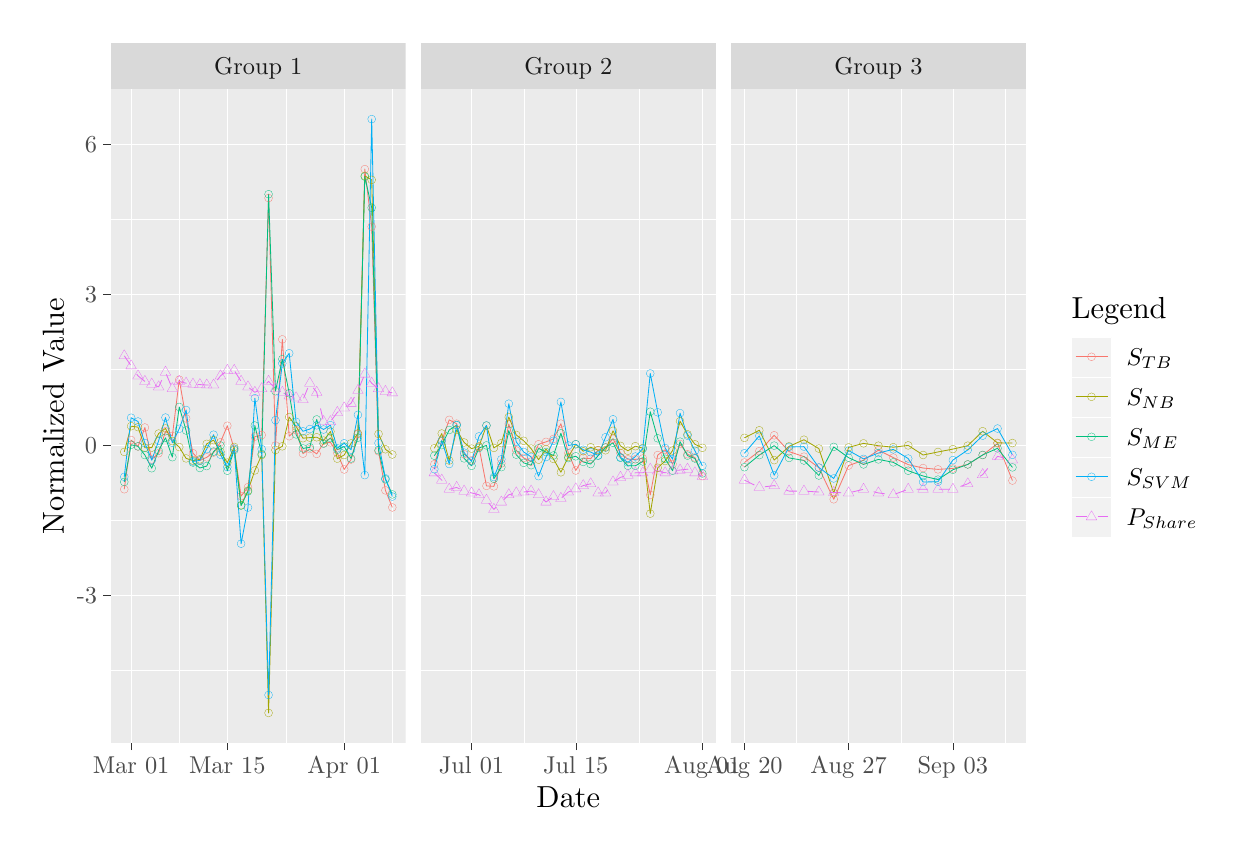
\begin{tikzpicture}[x=1pt,y=1pt]
\definecolor{fillColor}{RGB}{255,255,255}
\path[use as bounding box,fill=fillColor,fill opacity=0.00] (0,0) rectangle (433.62,289.08);
\begin{scope}
\path[clip] (  0.00,  0.00) rectangle (433.62,289.08);
\definecolor{drawColor}{RGB}{255,255,255}
\definecolor{fillColor}{RGB}{255,255,255}

\path[draw=drawColor,line width= 0.1pt,line join=round,line cap=round,fill=fillColor] (  0.00,  0.00) rectangle (433.62,289.08);
\end{scope}
\begin{scope}
\path[clip] ( 30.06, 30.73) rectangle (136.60,266.77);
\definecolor{fillColor}{gray}{0.92}

\path[fill=fillColor] ( 30.06, 30.73) rectangle (136.60,266.77);
\definecolor{drawColor}{RGB}{255,255,255}

\path[draw=drawColor,line width= 0.1pt,line join=round] ( 30.06, 56.94) --
	(136.60, 56.94);

\path[draw=drawColor,line width= 0.1pt,line join=round] ( 30.06,111.24) --
	(136.60,111.24);

\path[draw=drawColor,line width= 0.1pt,line join=round] ( 30.06,165.53) --
	(136.60,165.53);

\path[draw=drawColor,line width= 0.1pt,line join=round] ( 30.06,219.83) --
	(136.60,219.83);

\path[draw=drawColor,line width= 0.1pt,line join=round] ( 54.77, 30.73) --
	( 54.77,266.77);

\path[draw=drawColor,line width= 0.1pt,line join=round] ( 93.26, 30.73) --
	( 93.26,266.77);

\path[draw=drawColor,line width= 0.1pt,line join=round] (131.76, 30.73) --
	(131.76,266.77);

\path[draw=drawColor,line width= 0.1pt,line join=round] ( 30.06, 84.09) --
	(136.60, 84.09);

\path[draw=drawColor,line width= 0.1pt,line join=round] ( 30.06,138.38) --
	(136.60,138.38);

\path[draw=drawColor,line width= 0.1pt,line join=round] ( 30.06,192.68) --
	(136.60,192.68);

\path[draw=drawColor,line width= 0.1pt,line join=round] ( 30.06,246.98) --
	(136.60,246.98);

\path[draw=drawColor,line width= 0.1pt,line join=round] ( 37.38, 30.73) --
	( 37.38,266.77);

\path[draw=drawColor,line width= 0.1pt,line join=round] ( 72.15, 30.73) --
	( 72.15,266.77);

\path[draw=drawColor,line width= 0.1pt,line join=round] (114.37, 30.73) --
	(114.37,266.77);
\definecolor{drawColor}{RGB}{248,118,109}

\path[draw=drawColor,line width= 0.3pt,line join=round] ( 34.90,122.29) --
	( 37.38,140.08) --
	( 39.87,137.74) --
	( 42.35,144.59) --
	( 44.83,133.03) --
	( 47.32,135.31) --
	( 49.80,143.23) --
	( 52.28,141.55) --
	( 54.77,161.86) --
	( 57.25,147.90) --
	( 59.73,135.32) --
	( 62.22,132.68) --
	( 64.70,133.83) --
	( 67.18,135.55) --
	( 69.67,139.26) --
	( 72.15,145.23) --
	( 74.63,136.85) --
	( 77.12,119.81) --
	( 79.60,123.04) --
	( 82.09,141.30) --
	( 84.57,141.87) --
	( 87.05,227.52) --
	( 89.54,138.12) --
	( 92.02,176.45) --
	( 94.50,141.46) --
	( 96.99,143.64) --
	( 99.47,135.15) --
	(101.95,136.82) --
	(104.44,135.06) --
	(106.92,138.90) --
	(109.40,139.25) --
	(111.89,135.37) --
	(114.37,129.44) --
	(116.85,133.04) --
	(119.34,142.23) --
	(121.82,237.97) --
	(124.31,217.18) --
	(126.79,135.99) --
	(129.27,121.89) --
	(131.76,115.72);
\definecolor{drawColor}{RGB}{163,165,0}

\path[draw=drawColor,line width= 0.3pt,line join=round] ( 34.90,135.78) --
	( 37.38,145.08) --
	( 39.87,144.73) --
	( 42.35,137.30) --
	( 44.83,137.32) --
	( 47.32,142.41) --
	( 49.80,144.27) --
	( 52.28,139.70) --
	( 54.77,137.53) --
	( 57.25,133.44) --
	( 59.73,132.63) --
	( 62.22,133.10) --
	( 64.70,138.69) --
	( 67.18,140.05) --
	( 69.67,135.79) --
	( 72.15,131.89) --
	( 74.63,137.57) --
	( 77.12,116.53) --
	( 79.60,121.79) --
	( 82.09,129.10) --
	( 84.57,134.66) --
	( 87.05, 41.46) --
	( 89.54,136.47) --
	( 92.02,137.81) --
	( 94.50,148.38) --
	( 96.99,145.00) --
	( 99.47,140.73) --
	(101.95,140.94) --
	(104.44,141.08) --
	(106.92,139.87) --
	(109.40,143.17) --
	(111.89,133.34) --
	(114.37,134.66) --
	(116.85,138.86) --
	(119.34,142.45) --
	(121.82,235.52) --
	(124.31,234.08) --
	(126.79,142.26) --
	(129.27,136.74) --
	(131.76,134.85);
\definecolor{drawColor}{RGB}{0,191,125}

\path[draw=drawColor,line width= 0.3pt,line join=round] ( 34.90,124.93) --
	( 37.38,138.36) --
	( 39.87,137.80) --
	( 42.35,134.65) --
	( 44.83,129.88) --
	( 47.32,136.23) --
	( 49.80,140.89) --
	( 52.28,133.88) --
	( 54.77,152.02) --
	( 57.25,143.52) --
	( 59.73,131.94) --
	( 62.22,129.97) --
	( 64.70,130.66) --
	( 67.18,135.90) --
	( 69.67,138.09) --
	( 72.15,128.97) --
	( 74.63,136.46) --
	( 77.12,116.40) --
	( 79.60,121.52) --
	( 82.09,145.30) --
	( 84.57,135.03) --
	( 87.05,228.90) --
	( 89.54,157.72) --
	( 92.02,169.30) --
	( 94.50,156.97) --
	( 96.99,142.12) --
	( 99.47,137.04) --
	(101.95,137.43) --
	(104.44,147.52) --
	(106.92,138.77) --
	(109.40,140.80) --
	(111.89,136.58) --
	(114.37,137.74) --
	(116.85,133.40) --
	(119.34,140.92) --
	(121.82,235.26) --
	(124.31,224.02) --
	(126.79,136.41) --
	(129.27,125.87) --
	(131.76,120.43);
\definecolor{drawColor}{RGB}{0,176,246}

\path[draw=drawColor,line width= 0.3pt,line join=round] ( 34.90,126.77) --
	( 37.38,148.12) --
	( 39.87,146.76) --
	( 42.35,138.98) --
	( 44.83,132.78) --
	( 47.32,139.80) --
	( 49.80,148.19) --
	( 52.28,139.09) --
	( 54.77,144.13) --
	( 57.25,150.92) --
	( 59.73,132.32) --
	( 62.22,132.71) --
	( 64.70,136.81) --
	( 67.18,142.00) --
	( 69.67,134.77) --
	( 72.15,130.28) --
	( 74.63,136.98) --
	( 77.12,102.61) --
	( 79.60,115.66) --
	( 82.09,155.19) --
	( 84.57,136.80) --
	( 87.05, 47.94) --
	( 89.54,147.26) --
	( 92.02,167.78) --
	( 94.50,171.44) --
	( 96.99,146.64) --
	( 99.47,143.23) --
	(101.95,144.04) --
	(104.44,145.40) --
	(106.92,143.88) --
	(109.40,145.45) --
	(111.89,137.09) --
	(114.37,138.90) --
	(116.85,136.58) --
	(119.34,149.17) --
	(121.82,127.40) --
	(124.31,256.04) --
	(126.79,138.98) --
	(129.27,126.23) --
	(131.76,119.65);
\definecolor{drawColor}{RGB}{231,107,243}

\path[draw=drawColor,line width= 0.3pt,dash pattern=on 4pt off 4pt ,line join=round] ( 34.90,170.52) --
	( 37.38,166.89) --
	( 39.87,163.25) --
	( 42.35,161.27) --
	( 44.83,160.28) --
	( 47.32,159.29) --
	( 49.80,164.57) --
	( 52.28,158.63) --
	( 54.77,161.27) --
	( 57.25,160.61) --
	( 59.73,160.28) --
	( 62.22,160.11) --
	( 64.70,159.95) --
	( 67.18,159.95) --
	( 69.67,163.25) --
	( 72.15,165.24) --
	( 74.63,165.24) --
	( 77.12,161.27) --
	( 79.60,159.29) --
	( 82.09,157.31) --
	( 84.57,158.63) --
	( 87.05,161.27) --
	( 89.54,158.63) --
	( 92.02,157.31) --
	( 94.50,155.98) --
	( 96.99,155.32) --
	( 99.47,154.66) --
	(101.95,160.61) --
	(104.44,157.31) --
	(106.92,146.73) --
	(109.40,146.73) --
	(111.89,150.04) --
	(114.37,151.69) --
	(116.85,153.34) --
	(119.34,157.97) --
	(121.82,163.91) --
	(124.31,160.61) --
	(126.79,158.63) --
	(129.27,157.64) --
	(131.76,157.14);
\definecolor{drawColor}{RGB}{248,118,109}

\path[draw=drawColor,line width= 0.1pt,line join=round,line cap=round] ( 34.90,122.29) circle (  1.43);

\path[draw=drawColor,line width= 0.1pt,line join=round,line cap=round] ( 37.38,140.08) circle (  1.43);

\path[draw=drawColor,line width= 0.1pt,line join=round,line cap=round] ( 39.87,137.74) circle (  1.43);

\path[draw=drawColor,line width= 0.1pt,line join=round,line cap=round] ( 42.35,144.59) circle (  1.43);

\path[draw=drawColor,line width= 0.1pt,line join=round,line cap=round] ( 44.83,133.03) circle (  1.43);

\path[draw=drawColor,line width= 0.1pt,line join=round,line cap=round] ( 47.32,135.31) circle (  1.43);

\path[draw=drawColor,line width= 0.1pt,line join=round,line cap=round] ( 49.80,143.23) circle (  1.43);

\path[draw=drawColor,line width= 0.1pt,line join=round,line cap=round] ( 52.28,141.55) circle (  1.43);

\path[draw=drawColor,line width= 0.1pt,line join=round,line cap=round] ( 54.77,161.86) circle (  1.43);

\path[draw=drawColor,line width= 0.1pt,line join=round,line cap=round] ( 57.25,147.90) circle (  1.43);

\path[draw=drawColor,line width= 0.1pt,line join=round,line cap=round] ( 59.73,135.32) circle (  1.43);

\path[draw=drawColor,line width= 0.1pt,line join=round,line cap=round] ( 62.22,132.68) circle (  1.43);

\path[draw=drawColor,line width= 0.1pt,line join=round,line cap=round] ( 64.70,133.83) circle (  1.43);

\path[draw=drawColor,line width= 0.1pt,line join=round,line cap=round] ( 67.18,135.55) circle (  1.43);

\path[draw=drawColor,line width= 0.1pt,line join=round,line cap=round] ( 69.67,139.26) circle (  1.43);

\path[draw=drawColor,line width= 0.1pt,line join=round,line cap=round] ( 72.15,145.23) circle (  1.43);

\path[draw=drawColor,line width= 0.1pt,line join=round,line cap=round] ( 74.63,136.85) circle (  1.43);

\path[draw=drawColor,line width= 0.1pt,line join=round,line cap=round] ( 77.12,119.81) circle (  1.43);

\path[draw=drawColor,line width= 0.1pt,line join=round,line cap=round] ( 79.60,123.04) circle (  1.43);

\path[draw=drawColor,line width= 0.1pt,line join=round,line cap=round] ( 82.09,141.30) circle (  1.43);

\path[draw=drawColor,line width= 0.1pt,line join=round,line cap=round] ( 84.57,141.87) circle (  1.43);

\path[draw=drawColor,line width= 0.1pt,line join=round,line cap=round] ( 87.05,227.52) circle (  1.43);

\path[draw=drawColor,line width= 0.1pt,line join=round,line cap=round] ( 89.54,138.12) circle (  1.43);

\path[draw=drawColor,line width= 0.1pt,line join=round,line cap=round] ( 92.02,176.45) circle (  1.43);

\path[draw=drawColor,line width= 0.1pt,line join=round,line cap=round] ( 94.50,141.46) circle (  1.43);

\path[draw=drawColor,line width= 0.1pt,line join=round,line cap=round] ( 96.99,143.64) circle (  1.43);

\path[draw=drawColor,line width= 0.1pt,line join=round,line cap=round] ( 99.47,135.15) circle (  1.43);

\path[draw=drawColor,line width= 0.1pt,line join=round,line cap=round] (101.95,136.82) circle (  1.43);

\path[draw=drawColor,line width= 0.1pt,line join=round,line cap=round] (104.44,135.06) circle (  1.43);

\path[draw=drawColor,line width= 0.1pt,line join=round,line cap=round] (106.92,138.90) circle (  1.43);

\path[draw=drawColor,line width= 0.1pt,line join=round,line cap=round] (109.40,139.25) circle (  1.43);

\path[draw=drawColor,line width= 0.1pt,line join=round,line cap=round] (111.89,135.37) circle (  1.43);

\path[draw=drawColor,line width= 0.1pt,line join=round,line cap=round] (114.37,129.44) circle (  1.43);

\path[draw=drawColor,line width= 0.1pt,line join=round,line cap=round] (116.85,133.04) circle (  1.43);

\path[draw=drawColor,line width= 0.1pt,line join=round,line cap=round] (119.34,142.23) circle (  1.43);

\path[draw=drawColor,line width= 0.1pt,line join=round,line cap=round] (121.82,237.97) circle (  1.43);

\path[draw=drawColor,line width= 0.1pt,line join=round,line cap=round] (124.31,217.18) circle (  1.43);

\path[draw=drawColor,line width= 0.1pt,line join=round,line cap=round] (126.79,135.99) circle (  1.43);

\path[draw=drawColor,line width= 0.1pt,line join=round,line cap=round] (129.27,121.89) circle (  1.43);

\path[draw=drawColor,line width= 0.1pt,line join=round,line cap=round] (131.76,115.72) circle (  1.43);
\definecolor{drawColor}{RGB}{163,165,0}

\path[draw=drawColor,line width= 0.1pt,line join=round,line cap=round] ( 34.90,135.78) circle (  1.43);

\path[draw=drawColor,line width= 0.1pt,line join=round,line cap=round] ( 37.38,145.08) circle (  1.43);

\path[draw=drawColor,line width= 0.1pt,line join=round,line cap=round] ( 39.87,144.73) circle (  1.43);

\path[draw=drawColor,line width= 0.1pt,line join=round,line cap=round] ( 42.35,137.30) circle (  1.43);

\path[draw=drawColor,line width= 0.1pt,line join=round,line cap=round] ( 44.83,137.32) circle (  1.43);

\path[draw=drawColor,line width= 0.1pt,line join=round,line cap=round] ( 47.32,142.41) circle (  1.43);

\path[draw=drawColor,line width= 0.1pt,line join=round,line cap=round] ( 49.80,144.27) circle (  1.43);

\path[draw=drawColor,line width= 0.1pt,line join=round,line cap=round] ( 52.28,139.70) circle (  1.43);

\path[draw=drawColor,line width= 0.1pt,line join=round,line cap=round] ( 54.77,137.53) circle (  1.43);

\path[draw=drawColor,line width= 0.1pt,line join=round,line cap=round] ( 57.25,133.44) circle (  1.43);

\path[draw=drawColor,line width= 0.1pt,line join=round,line cap=round] ( 59.73,132.63) circle (  1.43);

\path[draw=drawColor,line width= 0.1pt,line join=round,line cap=round] ( 62.22,133.10) circle (  1.43);

\path[draw=drawColor,line width= 0.1pt,line join=round,line cap=round] ( 64.70,138.69) circle (  1.43);

\path[draw=drawColor,line width= 0.1pt,line join=round,line cap=round] ( 67.18,140.05) circle (  1.43);

\path[draw=drawColor,line width= 0.1pt,line join=round,line cap=round] ( 69.67,135.79) circle (  1.43);

\path[draw=drawColor,line width= 0.1pt,line join=round,line cap=round] ( 72.15,131.89) circle (  1.43);

\path[draw=drawColor,line width= 0.1pt,line join=round,line cap=round] ( 74.63,137.57) circle (  1.43);

\path[draw=drawColor,line width= 0.1pt,line join=round,line cap=round] ( 77.12,116.53) circle (  1.43);

\path[draw=drawColor,line width= 0.1pt,line join=round,line cap=round] ( 79.60,121.79) circle (  1.43);

\path[draw=drawColor,line width= 0.1pt,line join=round,line cap=round] ( 82.09,129.10) circle (  1.43);

\path[draw=drawColor,line width= 0.1pt,line join=round,line cap=round] ( 84.57,134.66) circle (  1.43);

\path[draw=drawColor,line width= 0.1pt,line join=round,line cap=round] ( 87.05, 41.46) circle (  1.43);

\path[draw=drawColor,line width= 0.1pt,line join=round,line cap=round] ( 89.54,136.47) circle (  1.43);

\path[draw=drawColor,line width= 0.1pt,line join=round,line cap=round] ( 92.02,137.81) circle (  1.43);

\path[draw=drawColor,line width= 0.1pt,line join=round,line cap=round] ( 94.50,148.38) circle (  1.43);

\path[draw=drawColor,line width= 0.1pt,line join=round,line cap=round] ( 96.99,145.00) circle (  1.43);

\path[draw=drawColor,line width= 0.1pt,line join=round,line cap=round] ( 99.47,140.73) circle (  1.43);

\path[draw=drawColor,line width= 0.1pt,line join=round,line cap=round] (101.95,140.94) circle (  1.43);

\path[draw=drawColor,line width= 0.1pt,line join=round,line cap=round] (104.44,141.08) circle (  1.43);

\path[draw=drawColor,line width= 0.1pt,line join=round,line cap=round] (106.92,139.87) circle (  1.43);

\path[draw=drawColor,line width= 0.1pt,line join=round,line cap=round] (109.40,143.17) circle (  1.43);

\path[draw=drawColor,line width= 0.1pt,line join=round,line cap=round] (111.89,133.34) circle (  1.43);

\path[draw=drawColor,line width= 0.1pt,line join=round,line cap=round] (114.37,134.66) circle (  1.43);

\path[draw=drawColor,line width= 0.1pt,line join=round,line cap=round] (116.85,138.86) circle (  1.43);

\path[draw=drawColor,line width= 0.1pt,line join=round,line cap=round] (119.34,142.45) circle (  1.43);

\path[draw=drawColor,line width= 0.1pt,line join=round,line cap=round] (121.82,235.52) circle (  1.43);

\path[draw=drawColor,line width= 0.1pt,line join=round,line cap=round] (124.31,234.08) circle (  1.43);

\path[draw=drawColor,line width= 0.1pt,line join=round,line cap=round] (126.79,142.26) circle (  1.43);

\path[draw=drawColor,line width= 0.1pt,line join=round,line cap=round] (129.27,136.74) circle (  1.43);

\path[draw=drawColor,line width= 0.1pt,line join=round,line cap=round] (131.76,134.85) circle (  1.43);
\definecolor{drawColor}{RGB}{0,191,125}

\path[draw=drawColor,line width= 0.1pt,line join=round,line cap=round] ( 34.90,124.93) circle (  1.43);

\path[draw=drawColor,line width= 0.1pt,line join=round,line cap=round] ( 37.38,138.36) circle (  1.43);

\path[draw=drawColor,line width= 0.1pt,line join=round,line cap=round] ( 39.87,137.80) circle (  1.43);

\path[draw=drawColor,line width= 0.1pt,line join=round,line cap=round] ( 42.35,134.65) circle (  1.43);

\path[draw=drawColor,line width= 0.1pt,line join=round,line cap=round] ( 44.83,129.88) circle (  1.43);

\path[draw=drawColor,line width= 0.1pt,line join=round,line cap=round] ( 47.32,136.23) circle (  1.43);

\path[draw=drawColor,line width= 0.1pt,line join=round,line cap=round] ( 49.80,140.89) circle (  1.43);

\path[draw=drawColor,line width= 0.1pt,line join=round,line cap=round] ( 52.28,133.88) circle (  1.43);

\path[draw=drawColor,line width= 0.1pt,line join=round,line cap=round] ( 54.77,152.02) circle (  1.43);

\path[draw=drawColor,line width= 0.1pt,line join=round,line cap=round] ( 57.25,143.52) circle (  1.43);

\path[draw=drawColor,line width= 0.1pt,line join=round,line cap=round] ( 59.73,131.94) circle (  1.43);

\path[draw=drawColor,line width= 0.1pt,line join=round,line cap=round] ( 62.22,129.97) circle (  1.43);

\path[draw=drawColor,line width= 0.1pt,line join=round,line cap=round] ( 64.70,130.66) circle (  1.43);

\path[draw=drawColor,line width= 0.1pt,line join=round,line cap=round] ( 67.18,135.90) circle (  1.43);

\path[draw=drawColor,line width= 0.1pt,line join=round,line cap=round] ( 69.67,138.09) circle (  1.43);

\path[draw=drawColor,line width= 0.1pt,line join=round,line cap=round] ( 72.15,128.97) circle (  1.43);

\path[draw=drawColor,line width= 0.1pt,line join=round,line cap=round] ( 74.63,136.46) circle (  1.43);

\path[draw=drawColor,line width= 0.1pt,line join=round,line cap=round] ( 77.12,116.40) circle (  1.43);

\path[draw=drawColor,line width= 0.1pt,line join=round,line cap=round] ( 79.60,121.52) circle (  1.43);

\path[draw=drawColor,line width= 0.1pt,line join=round,line cap=round] ( 82.09,145.30) circle (  1.43);

\path[draw=drawColor,line width= 0.1pt,line join=round,line cap=round] ( 84.57,135.03) circle (  1.43);

\path[draw=drawColor,line width= 0.1pt,line join=round,line cap=round] ( 87.05,228.90) circle (  1.43);

\path[draw=drawColor,line width= 0.1pt,line join=round,line cap=round] ( 89.54,157.72) circle (  1.43);

\path[draw=drawColor,line width= 0.1pt,line join=round,line cap=round] ( 92.02,169.30) circle (  1.43);

\path[draw=drawColor,line width= 0.1pt,line join=round,line cap=round] ( 94.50,156.97) circle (  1.43);

\path[draw=drawColor,line width= 0.1pt,line join=round,line cap=round] ( 96.99,142.12) circle (  1.43);

\path[draw=drawColor,line width= 0.1pt,line join=round,line cap=round] ( 99.47,137.04) circle (  1.43);

\path[draw=drawColor,line width= 0.1pt,line join=round,line cap=round] (101.95,137.43) circle (  1.43);

\path[draw=drawColor,line width= 0.1pt,line join=round,line cap=round] (104.44,147.52) circle (  1.43);

\path[draw=drawColor,line width= 0.1pt,line join=round,line cap=round] (106.92,138.77) circle (  1.43);

\path[draw=drawColor,line width= 0.1pt,line join=round,line cap=round] (109.40,140.80) circle (  1.43);

\path[draw=drawColor,line width= 0.1pt,line join=round,line cap=round] (111.89,136.58) circle (  1.43);

\path[draw=drawColor,line width= 0.1pt,line join=round,line cap=round] (114.37,137.74) circle (  1.43);

\path[draw=drawColor,line width= 0.1pt,line join=round,line cap=round] (116.85,133.40) circle (  1.43);

\path[draw=drawColor,line width= 0.1pt,line join=round,line cap=round] (119.34,140.92) circle (  1.43);

\path[draw=drawColor,line width= 0.1pt,line join=round,line cap=round] (121.82,235.26) circle (  1.43);

\path[draw=drawColor,line width= 0.1pt,line join=round,line cap=round] (124.31,224.02) circle (  1.43);

\path[draw=drawColor,line width= 0.1pt,line join=round,line cap=round] (126.79,136.41) circle (  1.43);

\path[draw=drawColor,line width= 0.1pt,line join=round,line cap=round] (129.27,125.87) circle (  1.43);

\path[draw=drawColor,line width= 0.1pt,line join=round,line cap=round] (131.76,120.43) circle (  1.43);
\definecolor{drawColor}{RGB}{0,176,246}

\path[draw=drawColor,line width= 0.1pt,line join=round,line cap=round] ( 34.90,126.77) circle (  1.43);

\path[draw=drawColor,line width= 0.1pt,line join=round,line cap=round] ( 37.38,148.12) circle (  1.43);

\path[draw=drawColor,line width= 0.1pt,line join=round,line cap=round] ( 39.87,146.76) circle (  1.43);

\path[draw=drawColor,line width= 0.1pt,line join=round,line cap=round] ( 42.35,138.98) circle (  1.43);

\path[draw=drawColor,line width= 0.1pt,line join=round,line cap=round] ( 44.83,132.78) circle (  1.43);

\path[draw=drawColor,line width= 0.1pt,line join=round,line cap=round] ( 47.32,139.80) circle (  1.43);

\path[draw=drawColor,line width= 0.1pt,line join=round,line cap=round] ( 49.80,148.19) circle (  1.43);

\path[draw=drawColor,line width= 0.1pt,line join=round,line cap=round] ( 52.28,139.09) circle (  1.43);

\path[draw=drawColor,line width= 0.1pt,line join=round,line cap=round] ( 54.77,144.13) circle (  1.43);

\path[draw=drawColor,line width= 0.1pt,line join=round,line cap=round] ( 57.25,150.92) circle (  1.43);

\path[draw=drawColor,line width= 0.1pt,line join=round,line cap=round] ( 59.73,132.32) circle (  1.43);

\path[draw=drawColor,line width= 0.1pt,line join=round,line cap=round] ( 62.22,132.71) circle (  1.43);

\path[draw=drawColor,line width= 0.1pt,line join=round,line cap=round] ( 64.70,136.81) circle (  1.43);

\path[draw=drawColor,line width= 0.1pt,line join=round,line cap=round] ( 67.18,142.00) circle (  1.43);

\path[draw=drawColor,line width= 0.1pt,line join=round,line cap=round] ( 69.67,134.77) circle (  1.43);

\path[draw=drawColor,line width= 0.1pt,line join=round,line cap=round] ( 72.15,130.28) circle (  1.43);

\path[draw=drawColor,line width= 0.1pt,line join=round,line cap=round] ( 74.63,136.98) circle (  1.43);

\path[draw=drawColor,line width= 0.1pt,line join=round,line cap=round] ( 77.12,102.61) circle (  1.43);

\path[draw=drawColor,line width= 0.1pt,line join=round,line cap=round] ( 79.60,115.66) circle (  1.43);

\path[draw=drawColor,line width= 0.1pt,line join=round,line cap=round] ( 82.09,155.19) circle (  1.43);

\path[draw=drawColor,line width= 0.1pt,line join=round,line cap=round] ( 84.57,136.80) circle (  1.43);

\path[draw=drawColor,line width= 0.1pt,line join=round,line cap=round] ( 87.05, 47.94) circle (  1.43);

\path[draw=drawColor,line width= 0.1pt,line join=round,line cap=round] ( 89.54,147.26) circle (  1.43);

\path[draw=drawColor,line width= 0.1pt,line join=round,line cap=round] ( 92.02,167.78) circle (  1.43);

\path[draw=drawColor,line width= 0.1pt,line join=round,line cap=round] ( 94.50,171.44) circle (  1.43);

\path[draw=drawColor,line width= 0.1pt,line join=round,line cap=round] ( 96.99,146.64) circle (  1.43);

\path[draw=drawColor,line width= 0.1pt,line join=round,line cap=round] ( 99.47,143.23) circle (  1.43);

\path[draw=drawColor,line width= 0.1pt,line join=round,line cap=round] (101.95,144.04) circle (  1.43);

\path[draw=drawColor,line width= 0.1pt,line join=round,line cap=round] (104.44,145.40) circle (  1.43);

\path[draw=drawColor,line width= 0.1pt,line join=round,line cap=round] (106.92,143.88) circle (  1.43);

\path[draw=drawColor,line width= 0.1pt,line join=round,line cap=round] (109.40,145.45) circle (  1.43);

\path[draw=drawColor,line width= 0.1pt,line join=round,line cap=round] (111.89,137.09) circle (  1.43);

\path[draw=drawColor,line width= 0.1pt,line join=round,line cap=round] (114.37,138.90) circle (  1.43);

\path[draw=drawColor,line width= 0.1pt,line join=round,line cap=round] (116.85,136.58) circle (  1.43);

\path[draw=drawColor,line width= 0.1pt,line join=round,line cap=round] (119.34,149.17) circle (  1.43);

\path[draw=drawColor,line width= 0.1pt,line join=round,line cap=round] (121.82,127.40) circle (  1.43);

\path[draw=drawColor,line width= 0.1pt,line join=round,line cap=round] (124.31,256.04) circle (  1.43);

\path[draw=drawColor,line width= 0.1pt,line join=round,line cap=round] (126.79,138.98) circle (  1.43);

\path[draw=drawColor,line width= 0.1pt,line join=round,line cap=round] (129.27,126.23) circle (  1.43);

\path[draw=drawColor,line width= 0.1pt,line join=round,line cap=round] (131.76,119.65) circle (  1.43);
\definecolor{drawColor}{RGB}{231,107,243}

\path[draw=drawColor,line width= 0.1pt,line join=round,line cap=round] ( 34.90,172.74) --
	( 36.82,169.41) --
	( 32.98,169.41) --
	( 34.90,172.74);

\path[draw=drawColor,line width= 0.1pt,line join=round,line cap=round] ( 37.38,169.11) --
	( 39.30,165.78) --
	( 35.46,165.78) --
	( 37.38,169.11);

\path[draw=drawColor,line width= 0.1pt,line join=round,line cap=round] ( 39.87,165.47) --
	( 41.79,162.14) --
	( 37.94,162.14) --
	( 39.87,165.47);

\path[draw=drawColor,line width= 0.1pt,line join=round,line cap=round] ( 42.35,163.49) --
	( 44.27,160.16) --
	( 40.43,160.16) --
	( 42.35,163.49);

\path[draw=drawColor,line width= 0.1pt,line join=round,line cap=round] ( 44.83,162.50) --
	( 46.75,159.17) --
	( 42.91,159.17) --
	( 44.83,162.50);

\path[draw=drawColor,line width= 0.1pt,line join=round,line cap=round] ( 47.32,161.51) --
	( 49.24,158.18) --
	( 45.39,158.18) --
	( 47.32,161.51);

\path[draw=drawColor,line width= 0.1pt,line join=round,line cap=round] ( 49.80,166.79) --
	( 51.72,163.47) --
	( 47.88,163.47) --
	( 49.80,166.79);

\path[draw=drawColor,line width= 0.1pt,line join=round,line cap=round] ( 52.28,160.85) --
	( 54.20,157.52) --
	( 50.36,157.52) --
	( 52.28,160.85);

\path[draw=drawColor,line width= 0.1pt,line join=round,line cap=round] ( 54.77,163.49) --
	( 56.69,160.16) --
	( 52.85,160.16) --
	( 54.77,163.49);

\path[draw=drawColor,line width= 0.1pt,line join=round,line cap=round] ( 57.25,162.83) --
	( 59.17,159.50) --
	( 55.33,159.50) --
	( 57.25,162.83);

\path[draw=drawColor,line width= 0.1pt,line join=round,line cap=round] ( 59.73,162.50) --
	( 61.65,159.17) --
	( 57.81,159.17) --
	( 59.73,162.50);

\path[draw=drawColor,line width= 0.1pt,line join=round,line cap=round] ( 62.22,162.33) --
	( 64.14,159.00) --
	( 60.30,159.00) --
	( 62.22,162.33);

\path[draw=drawColor,line width= 0.1pt,line join=round,line cap=round] ( 64.70,162.17) --
	( 66.62,158.84) --
	( 62.78,158.84) --
	( 64.70,162.17);

\path[draw=drawColor,line width= 0.1pt,line join=round,line cap=round] ( 67.18,162.17) --
	( 69.11,158.84) --
	( 65.26,158.84) --
	( 67.18,162.17);

\path[draw=drawColor,line width= 0.1pt,line join=round,line cap=round] ( 69.67,165.47) --
	( 71.59,162.14) --
	( 67.75,162.14) --
	( 69.67,165.47);

\path[draw=drawColor,line width= 0.1pt,line join=round,line cap=round] ( 72.15,167.45) --
	( 74.07,164.13) --
	( 70.23,164.13) --
	( 72.15,167.45);

\path[draw=drawColor,line width= 0.1pt,line join=round,line cap=round] ( 74.63,167.45) --
	( 76.56,164.13) --
	( 72.71,164.13) --
	( 74.63,167.45);

\path[draw=drawColor,line width= 0.1pt,line join=round,line cap=round] ( 77.12,163.49) --
	( 79.04,160.16) --
	( 75.20,160.16) --
	( 77.12,163.49);

\path[draw=drawColor,line width= 0.1pt,line join=round,line cap=round] ( 79.60,161.51) --
	( 81.52,158.18) --
	( 77.68,158.18) --
	( 79.60,161.51);

\path[draw=drawColor,line width= 0.1pt,line join=round,line cap=round] ( 82.09,159.52) --
	( 84.01,156.20) --
	( 80.16,156.20) --
	( 82.09,159.52);

\path[draw=drawColor,line width= 0.1pt,line join=round,line cap=round] ( 84.57,160.85) --
	( 86.49,157.52) --
	( 82.65,157.52) --
	( 84.57,160.85);

\path[draw=drawColor,line width= 0.1pt,line join=round,line cap=round] ( 87.05,163.49) --
	( 88.97,160.16) --
	( 85.13,160.16) --
	( 87.05,163.49);

\path[draw=drawColor,line width= 0.1pt,line join=round,line cap=round] ( 89.54,160.85) --
	( 91.46,157.52) --
	( 87.61,157.52) --
	( 89.54,160.85);

\path[draw=drawColor,line width= 0.1pt,line join=round,line cap=round] ( 92.02,159.52) --
	( 93.94,156.20) --
	( 90.10,156.20) --
	( 92.02,159.52);

\path[draw=drawColor,line width= 0.1pt,line join=round,line cap=round] ( 94.50,158.20) --
	( 96.42,154.87) --
	( 92.58,154.87) --
	( 94.50,158.20);

\path[draw=drawColor,line width= 0.1pt,line join=round,line cap=round] ( 96.99,157.54) --
	( 98.91,154.21) --
	( 95.07,154.21) --
	( 96.99,157.54);

\path[draw=drawColor,line width= 0.1pt,line join=round,line cap=round] ( 99.47,156.88) --
	(101.39,153.55) --
	( 97.55,153.55) --
	( 99.47,156.88);

\path[draw=drawColor,line width= 0.1pt,line join=round,line cap=round] (101.95,162.83) --
	(103.87,159.50) --
	(100.03,159.50) --
	(101.95,162.83);

\path[draw=drawColor,line width= 0.1pt,line join=round,line cap=round] (104.44,159.52) --
	(106.36,156.20) --
	(102.52,156.20) --
	(104.44,159.52);

\path[draw=drawColor,line width= 0.1pt,line join=round,line cap=round] (106.92,148.95) --
	(108.84,145.62) --
	(105.00,145.62) --
	(106.92,148.95);

\path[draw=drawColor,line width= 0.1pt,line join=round,line cap=round] (109.40,148.95) --
	(111.33,145.62) --
	(107.48,145.62) --
	(109.40,148.95);

\path[draw=drawColor,line width= 0.1pt,line join=round,line cap=round] (111.89,152.26) --
	(113.81,148.93) --
	(109.97,148.93) --
	(111.89,152.26);

\path[draw=drawColor,line width= 0.1pt,line join=round,line cap=round] (114.37,153.91) --
	(116.29,150.58) --
	(112.45,150.58) --
	(114.37,153.91);

\path[draw=drawColor,line width= 0.1pt,line join=round,line cap=round] (116.85,155.56) --
	(118.78,152.23) --
	(114.93,152.23) --
	(116.85,155.56);

\path[draw=drawColor,line width= 0.1pt,line join=round,line cap=round] (119.34,160.19) --
	(121.26,156.86) --
	(117.42,156.86) --
	(119.34,160.19);

\path[draw=drawColor,line width= 0.1pt,line join=round,line cap=round] (121.82,166.13) --
	(123.74,162.80) --
	(119.90,162.80) --
	(121.82,166.13);

\path[draw=drawColor,line width= 0.1pt,line join=round,line cap=round] (124.31,162.83) --
	(126.23,159.50) --
	(122.38,159.50) --
	(124.31,162.83);

\path[draw=drawColor,line width= 0.1pt,line join=round,line cap=round] (126.79,160.85) --
	(128.71,157.52) --
	(124.87,157.52) --
	(126.79,160.85);

\path[draw=drawColor,line width= 0.1pt,line join=round,line cap=round] (129.27,159.85) --
	(131.19,156.53) --
	(127.35,156.53) --
	(129.27,159.85);

\path[draw=drawColor,line width= 0.1pt,line join=round,line cap=round] (131.76,159.36) --
	(133.68,156.03) --
	(129.83,156.03) --
	(131.76,159.36);
\end{scope}
\begin{scope}
\path[clip] (142.10, 30.73) rectangle (248.64,266.77);
\definecolor{fillColor}{gray}{0.92}

\path[fill=fillColor] (142.10, 30.73) rectangle (248.64,266.77);
\definecolor{drawColor}{RGB}{255,255,255}

\path[draw=drawColor,line width= 0.1pt,line join=round] (142.10, 56.94) --
	(248.64, 56.94);

\path[draw=drawColor,line width= 0.1pt,line join=round] (142.10,111.24) --
	(248.64,111.24);

\path[draw=drawColor,line width= 0.1pt,line join=round] (142.10,165.53) --
	(248.64,165.53);

\path[draw=drawColor,line width= 0.1pt,line join=round] (142.10,219.83) --
	(248.64,219.83);

\path[draw=drawColor,line width= 0.1pt,line join=round] (179.23, 30.73) --
	(179.23,266.77);

\path[draw=drawColor,line width= 0.1pt,line join=round] (220.93, 30.73) --
	(220.93,266.77);

\path[draw=drawColor,line width= 0.1pt,line join=round] (142.10, 84.09) --
	(248.64, 84.09);

\path[draw=drawColor,line width= 0.1pt,line join=round] (142.10,138.38) --
	(248.64,138.38);

\path[draw=drawColor,line width= 0.1pt,line join=round] (142.10,192.68) --
	(248.64,192.68);

\path[draw=drawColor,line width= 0.1pt,line join=round] (142.10,246.98) --
	(248.64,246.98);

\path[draw=drawColor,line width= 0.1pt,line join=round] (160.39, 30.73) --
	(160.39,266.77);

\path[draw=drawColor,line width= 0.1pt,line join=round] (198.06, 30.73) --
	(198.06,266.77);

\path[draw=drawColor,line width= 0.1pt,line join=round] (243.80, 30.73) --
	(243.80,266.77);
\definecolor{drawColor}{RGB}{248,118,109}

\path[draw=drawColor,line width= 0.3pt,line join=round] (146.94,131.34) --
	(149.63,139.81) --
	(152.32,147.36) --
	(155.01,145.98) --
	(157.70,134.96) --
	(160.39,132.73) --
	(163.08,137.53) --
	(165.78,123.50) --
	(168.47,123.33) --
	(171.16,131.62) --
	(173.85,145.88) --
	(176.54,136.30) --
	(179.23,133.61) --
	(181.92,132.30) --
	(184.61,138.55) --
	(187.30,139.41) --
	(189.99,140.45) --
	(192.68,145.99) --
	(195.37,135.33) --
	(198.06,129.07) --
	(200.75,133.58) --
	(203.44,133.35) --
	(206.13,136.45) --
	(208.82,137.45) --
	(211.51,140.52) --
	(214.20,135.40) --
	(216.89,133.11) --
	(219.58,133.09) --
	(222.28,133.41) --
	(224.97,120.24) --
	(227.66,134.64) --
	(230.35,136.59) --
	(233.04,131.33) --
	(235.73,138.64) --
	(238.42,134.94) --
	(241.11,133.74) --
	(243.80,127.02);
\definecolor{drawColor}{RGB}{163,165,0}

\path[draw=drawColor,line width= 0.3pt,line join=round] (146.94,137.09) --
	(149.63,142.42) --
	(152.32,132.67) --
	(155.01,143.73) --
	(157.70,139.20) --
	(160.39,136.96) --
	(163.08,137.78) --
	(165.78,145.29) --
	(168.47,137.22) --
	(171.16,138.96) --
	(173.85,148.38) --
	(176.54,141.91) --
	(179.23,139.80) --
	(181.92,136.97) --
	(184.61,132.97) --
	(187.30,136.81) --
	(189.99,133.25) --
	(192.68,128.43) --
	(195.37,133.97) --
	(198.06,138.57) --
	(200.75,136.02) --
	(203.44,137.47) --
	(206.13,136.40) --
	(208.82,136.38) --
	(211.51,143.40) --
	(214.20,137.96) --
	(216.89,136.19) --
	(219.58,137.85) --
	(222.28,137.14) --
	(224.97,113.48) --
	(227.66,130.05) --
	(230.35,132.50) --
	(233.04,136.27) --
	(235.73,146.89) --
	(238.42,142.14) --
	(241.11,138.54) --
	(243.80,137.25);
\definecolor{drawColor}{RGB}{0,191,125}

\path[draw=drawColor,line width= 0.3pt,line join=round] (146.94,134.42) --
	(149.63,138.23) --
	(152.32,143.70) --
	(155.01,145.46) --
	(157.70,133.44) --
	(160.39,130.74) --
	(163.08,137.21) --
	(165.78,138.13) --
	(168.47,126.08) --
	(171.16,130.28) --
	(173.85,143.51) --
	(176.54,134.80) --
	(179.23,131.82) --
	(181.92,130.98) --
	(184.61,137.07) --
	(187.30,135.72) --
	(189.99,134.48) --
	(192.68,142.51) --
	(195.37,133.55) --
	(198.06,134.20) --
	(200.75,132.16) --
	(203.44,131.40) --
	(206.13,134.40) --
	(208.82,137.35) --
	(211.51,139.08) --
	(214.20,133.64) --
	(216.89,130.77) --
	(219.58,130.76) --
	(222.28,132.34) --
	(224.97,150.30) --
	(227.66,140.71) --
	(230.35,133.30) --
	(233.04,128.98) --
	(235.73,139.49) --
	(238.42,134.44) --
	(241.11,133.41) --
	(243.80,128.00);
\definecolor{drawColor}{RGB}{0,176,246}

\path[draw=drawColor,line width= 0.3pt,line join=round] (146.94,129.54) --
	(149.63,139.85) --
	(152.32,131.41) --
	(155.01,145.51) --
	(157.70,135.53) --
	(160.39,132.35) --
	(163.08,141.40) --
	(165.78,145.35) --
	(168.47,126.69) --
	(171.16,133.11) --
	(173.85,153.20) --
	(176.54,139.44) --
	(179.23,135.76) --
	(181.92,133.99) --
	(184.61,127.02) --
	(187.30,133.93) --
	(189.99,139.81) --
	(192.68,153.85) --
	(195.37,138.09) --
	(198.06,138.55) --
	(200.75,136.56) --
	(203.44,135.69) --
	(206.13,134.52) --
	(208.82,141.08) --
	(211.51,147.58) --
	(214.20,133.82) --
	(216.89,131.99) --
	(219.58,134.10) --
	(222.28,136.96) --
	(224.97,164.14) --
	(227.66,150.10) --
	(230.35,137.16) --
	(233.04,133.13) --
	(235.73,149.80) --
	(238.42,141.65) --
	(241.11,136.20) --
	(243.80,130.72);
\definecolor{drawColor}{RGB}{231,107,243}

\path[draw=drawColor,line width= 0.3pt,dash pattern=on 4pt off 4pt ,line join=round] (146.94,128.23) --
	(149.63,125.59) --
	(152.32,122.28) --
	(155.01,122.94) --
	(157.70,121.62) --
	(160.39,120.96) --
	(163.08,120.30) --
	(165.78,118.32) --
	(168.47,115.01) --
	(171.16,117.66) --
	(173.85,120.30) --
	(176.54,120.96) --
	(179.23,121.29) --
	(181.92,121.62) --
	(184.61,120.30) --
	(187.30,117.66) --
	(189.99,119.64) --
	(192.68,118.98) --
	(195.37,121.29) --
	(198.06,122.45) --
	(200.75,123.60) --
	(203.44,124.27) --
	(206.13,120.96) --
	(208.82,120.96) --
	(211.51,124.93) --
	(214.20,126.58) --
	(216.89,127.40) --
	(219.58,128.23) --
	(222.28,128.23) --
	(224.97,129.55) --
	(227.66,128.89) --
	(230.35,128.23) --
	(233.04,128.89) --
	(235.73,129.22) --
	(238.42,129.55) --
	(241.11,128.23) --
	(243.80,126.91);
\definecolor{drawColor}{RGB}{248,118,109}

\path[draw=drawColor,line width= 0.1pt,line join=round,line cap=round] (146.94,131.34) circle (  1.43);

\path[draw=drawColor,line width= 0.1pt,line join=round,line cap=round] (149.63,139.81) circle (  1.43);

\path[draw=drawColor,line width= 0.1pt,line join=round,line cap=round] (152.32,147.36) circle (  1.43);

\path[draw=drawColor,line width= 0.1pt,line join=round,line cap=round] (155.01,145.98) circle (  1.43);

\path[draw=drawColor,line width= 0.1pt,line join=round,line cap=round] (157.70,134.96) circle (  1.43);

\path[draw=drawColor,line width= 0.1pt,line join=round,line cap=round] (160.39,132.73) circle (  1.43);

\path[draw=drawColor,line width= 0.1pt,line join=round,line cap=round] (163.08,137.53) circle (  1.43);

\path[draw=drawColor,line width= 0.1pt,line join=round,line cap=round] (165.78,123.50) circle (  1.43);

\path[draw=drawColor,line width= 0.1pt,line join=round,line cap=round] (168.47,123.33) circle (  1.43);

\path[draw=drawColor,line width= 0.1pt,line join=round,line cap=round] (171.16,131.62) circle (  1.43);

\path[draw=drawColor,line width= 0.1pt,line join=round,line cap=round] (173.85,145.88) circle (  1.43);

\path[draw=drawColor,line width= 0.1pt,line join=round,line cap=round] (176.54,136.30) circle (  1.43);

\path[draw=drawColor,line width= 0.1pt,line join=round,line cap=round] (179.23,133.61) circle (  1.43);

\path[draw=drawColor,line width= 0.1pt,line join=round,line cap=round] (181.92,132.30) circle (  1.43);

\path[draw=drawColor,line width= 0.1pt,line join=round,line cap=round] (184.61,138.55) circle (  1.43);

\path[draw=drawColor,line width= 0.1pt,line join=round,line cap=round] (187.30,139.41) circle (  1.43);

\path[draw=drawColor,line width= 0.1pt,line join=round,line cap=round] (189.99,140.45) circle (  1.43);

\path[draw=drawColor,line width= 0.1pt,line join=round,line cap=round] (192.68,145.99) circle (  1.43);

\path[draw=drawColor,line width= 0.1pt,line join=round,line cap=round] (195.37,135.33) circle (  1.43);

\path[draw=drawColor,line width= 0.1pt,line join=round,line cap=round] (198.06,129.07) circle (  1.43);

\path[draw=drawColor,line width= 0.1pt,line join=round,line cap=round] (200.75,133.58) circle (  1.43);

\path[draw=drawColor,line width= 0.1pt,line join=round,line cap=round] (203.44,133.35) circle (  1.43);

\path[draw=drawColor,line width= 0.1pt,line join=round,line cap=round] (206.13,136.45) circle (  1.43);

\path[draw=drawColor,line width= 0.1pt,line join=round,line cap=round] (208.82,137.45) circle (  1.43);

\path[draw=drawColor,line width= 0.1pt,line join=round,line cap=round] (211.51,140.52) circle (  1.43);

\path[draw=drawColor,line width= 0.1pt,line join=round,line cap=round] (214.20,135.40) circle (  1.43);

\path[draw=drawColor,line width= 0.1pt,line join=round,line cap=round] (216.89,133.11) circle (  1.43);

\path[draw=drawColor,line width= 0.1pt,line join=round,line cap=round] (219.58,133.09) circle (  1.43);

\path[draw=drawColor,line width= 0.1pt,line join=round,line cap=round] (222.28,133.41) circle (  1.43);

\path[draw=drawColor,line width= 0.1pt,line join=round,line cap=round] (224.97,120.24) circle (  1.43);

\path[draw=drawColor,line width= 0.1pt,line join=round,line cap=round] (227.66,134.64) circle (  1.43);

\path[draw=drawColor,line width= 0.1pt,line join=round,line cap=round] (230.35,136.59) circle (  1.43);

\path[draw=drawColor,line width= 0.1pt,line join=round,line cap=round] (233.04,131.33) circle (  1.43);

\path[draw=drawColor,line width= 0.1pt,line join=round,line cap=round] (235.73,138.64) circle (  1.43);

\path[draw=drawColor,line width= 0.1pt,line join=round,line cap=round] (238.42,134.94) circle (  1.43);

\path[draw=drawColor,line width= 0.1pt,line join=round,line cap=round] (241.11,133.74) circle (  1.43);

\path[draw=drawColor,line width= 0.1pt,line join=round,line cap=round] (243.80,127.02) circle (  1.43);
\definecolor{drawColor}{RGB}{163,165,0}

\path[draw=drawColor,line width= 0.1pt,line join=round,line cap=round] (146.94,137.09) circle (  1.43);

\path[draw=drawColor,line width= 0.1pt,line join=round,line cap=round] (149.63,142.42) circle (  1.43);

\path[draw=drawColor,line width= 0.1pt,line join=round,line cap=round] (152.32,132.67) circle (  1.43);

\path[draw=drawColor,line width= 0.1pt,line join=round,line cap=round] (155.01,143.73) circle (  1.43);

\path[draw=drawColor,line width= 0.1pt,line join=round,line cap=round] (157.70,139.20) circle (  1.43);

\path[draw=drawColor,line width= 0.1pt,line join=round,line cap=round] (160.39,136.96) circle (  1.43);

\path[draw=drawColor,line width= 0.1pt,line join=round,line cap=round] (163.08,137.78) circle (  1.43);

\path[draw=drawColor,line width= 0.1pt,line join=round,line cap=round] (165.78,145.29) circle (  1.43);

\path[draw=drawColor,line width= 0.1pt,line join=round,line cap=round] (168.47,137.22) circle (  1.43);

\path[draw=drawColor,line width= 0.1pt,line join=round,line cap=round] (171.16,138.96) circle (  1.43);

\path[draw=drawColor,line width= 0.1pt,line join=round,line cap=round] (173.85,148.38) circle (  1.43);

\path[draw=drawColor,line width= 0.1pt,line join=round,line cap=round] (176.54,141.91) circle (  1.43);

\path[draw=drawColor,line width= 0.1pt,line join=round,line cap=round] (179.23,139.80) circle (  1.43);

\path[draw=drawColor,line width= 0.1pt,line join=round,line cap=round] (181.92,136.97) circle (  1.43);

\path[draw=drawColor,line width= 0.1pt,line join=round,line cap=round] (184.61,132.97) circle (  1.43);

\path[draw=drawColor,line width= 0.1pt,line join=round,line cap=round] (187.30,136.81) circle (  1.43);

\path[draw=drawColor,line width= 0.1pt,line join=round,line cap=round] (189.99,133.25) circle (  1.43);

\path[draw=drawColor,line width= 0.1pt,line join=round,line cap=round] (192.68,128.43) circle (  1.43);

\path[draw=drawColor,line width= 0.1pt,line join=round,line cap=round] (195.37,133.97) circle (  1.43);

\path[draw=drawColor,line width= 0.1pt,line join=round,line cap=round] (198.06,138.57) circle (  1.43);

\path[draw=drawColor,line width= 0.1pt,line join=round,line cap=round] (200.75,136.02) circle (  1.43);

\path[draw=drawColor,line width= 0.1pt,line join=round,line cap=round] (203.44,137.47) circle (  1.43);

\path[draw=drawColor,line width= 0.1pt,line join=round,line cap=round] (206.13,136.40) circle (  1.43);

\path[draw=drawColor,line width= 0.1pt,line join=round,line cap=round] (208.82,136.38) circle (  1.43);

\path[draw=drawColor,line width= 0.1pt,line join=round,line cap=round] (211.51,143.40) circle (  1.43);

\path[draw=drawColor,line width= 0.1pt,line join=round,line cap=round] (214.20,137.96) circle (  1.43);

\path[draw=drawColor,line width= 0.1pt,line join=round,line cap=round] (216.89,136.19) circle (  1.43);

\path[draw=drawColor,line width= 0.1pt,line join=round,line cap=round] (219.58,137.85) circle (  1.43);

\path[draw=drawColor,line width= 0.1pt,line join=round,line cap=round] (222.28,137.14) circle (  1.43);

\path[draw=drawColor,line width= 0.1pt,line join=round,line cap=round] (224.97,113.48) circle (  1.43);

\path[draw=drawColor,line width= 0.1pt,line join=round,line cap=round] (227.66,130.05) circle (  1.43);

\path[draw=drawColor,line width= 0.1pt,line join=round,line cap=round] (230.35,132.50) circle (  1.43);

\path[draw=drawColor,line width= 0.1pt,line join=round,line cap=round] (233.04,136.27) circle (  1.43);

\path[draw=drawColor,line width= 0.1pt,line join=round,line cap=round] (235.73,146.89) circle (  1.43);

\path[draw=drawColor,line width= 0.1pt,line join=round,line cap=round] (238.42,142.14) circle (  1.43);

\path[draw=drawColor,line width= 0.1pt,line join=round,line cap=round] (241.11,138.54) circle (  1.43);

\path[draw=drawColor,line width= 0.1pt,line join=round,line cap=round] (243.80,137.25) circle (  1.43);
\definecolor{drawColor}{RGB}{0,191,125}

\path[draw=drawColor,line width= 0.1pt,line join=round,line cap=round] (146.94,134.42) circle (  1.43);

\path[draw=drawColor,line width= 0.1pt,line join=round,line cap=round] (149.63,138.23) circle (  1.43);

\path[draw=drawColor,line width= 0.1pt,line join=round,line cap=round] (152.32,143.70) circle (  1.43);

\path[draw=drawColor,line width= 0.1pt,line join=round,line cap=round] (155.01,145.46) circle (  1.43);

\path[draw=drawColor,line width= 0.1pt,line join=round,line cap=round] (157.70,133.44) circle (  1.43);

\path[draw=drawColor,line width= 0.1pt,line join=round,line cap=round] (160.39,130.74) circle (  1.43);

\path[draw=drawColor,line width= 0.1pt,line join=round,line cap=round] (163.08,137.21) circle (  1.43);

\path[draw=drawColor,line width= 0.1pt,line join=round,line cap=round] (165.78,138.13) circle (  1.43);

\path[draw=drawColor,line width= 0.1pt,line join=round,line cap=round] (168.47,126.08) circle (  1.43);

\path[draw=drawColor,line width= 0.1pt,line join=round,line cap=round] (171.16,130.28) circle (  1.43);

\path[draw=drawColor,line width= 0.1pt,line join=round,line cap=round] (173.85,143.51) circle (  1.43);

\path[draw=drawColor,line width= 0.1pt,line join=round,line cap=round] (176.54,134.80) circle (  1.43);

\path[draw=drawColor,line width= 0.1pt,line join=round,line cap=round] (179.23,131.82) circle (  1.43);

\path[draw=drawColor,line width= 0.1pt,line join=round,line cap=round] (181.92,130.98) circle (  1.43);

\path[draw=drawColor,line width= 0.1pt,line join=round,line cap=round] (184.61,137.07) circle (  1.43);

\path[draw=drawColor,line width= 0.1pt,line join=round,line cap=round] (187.30,135.72) circle (  1.43);

\path[draw=drawColor,line width= 0.1pt,line join=round,line cap=round] (189.99,134.48) circle (  1.43);

\path[draw=drawColor,line width= 0.1pt,line join=round,line cap=round] (192.68,142.51) circle (  1.43);

\path[draw=drawColor,line width= 0.1pt,line join=round,line cap=round] (195.37,133.55) circle (  1.43);

\path[draw=drawColor,line width= 0.1pt,line join=round,line cap=round] (198.06,134.20) circle (  1.43);

\path[draw=drawColor,line width= 0.1pt,line join=round,line cap=round] (200.75,132.16) circle (  1.43);

\path[draw=drawColor,line width= 0.1pt,line join=round,line cap=round] (203.44,131.40) circle (  1.43);

\path[draw=drawColor,line width= 0.1pt,line join=round,line cap=round] (206.13,134.40) circle (  1.43);

\path[draw=drawColor,line width= 0.1pt,line join=round,line cap=round] (208.82,137.35) circle (  1.43);

\path[draw=drawColor,line width= 0.1pt,line join=round,line cap=round] (211.51,139.08) circle (  1.43);

\path[draw=drawColor,line width= 0.1pt,line join=round,line cap=round] (214.20,133.64) circle (  1.43);

\path[draw=drawColor,line width= 0.1pt,line join=round,line cap=round] (216.89,130.77) circle (  1.43);

\path[draw=drawColor,line width= 0.1pt,line join=round,line cap=round] (219.58,130.76) circle (  1.43);

\path[draw=drawColor,line width= 0.1pt,line join=round,line cap=round] (222.28,132.34) circle (  1.43);

\path[draw=drawColor,line width= 0.1pt,line join=round,line cap=round] (224.97,150.30) circle (  1.43);

\path[draw=drawColor,line width= 0.1pt,line join=round,line cap=round] (227.66,140.71) circle (  1.43);

\path[draw=drawColor,line width= 0.1pt,line join=round,line cap=round] (230.35,133.30) circle (  1.43);

\path[draw=drawColor,line width= 0.1pt,line join=round,line cap=round] (233.04,128.98) circle (  1.43);

\path[draw=drawColor,line width= 0.1pt,line join=round,line cap=round] (235.73,139.49) circle (  1.43);

\path[draw=drawColor,line width= 0.1pt,line join=round,line cap=round] (238.42,134.44) circle (  1.43);

\path[draw=drawColor,line width= 0.1pt,line join=round,line cap=round] (241.11,133.41) circle (  1.43);

\path[draw=drawColor,line width= 0.1pt,line join=round,line cap=round] (243.80,128.00) circle (  1.43);
\definecolor{drawColor}{RGB}{0,176,246}

\path[draw=drawColor,line width= 0.1pt,line join=round,line cap=round] (146.94,129.54) circle (  1.43);

\path[draw=drawColor,line width= 0.1pt,line join=round,line cap=round] (149.63,139.85) circle (  1.43);

\path[draw=drawColor,line width= 0.1pt,line join=round,line cap=round] (152.32,131.41) circle (  1.43);

\path[draw=drawColor,line width= 0.1pt,line join=round,line cap=round] (155.01,145.51) circle (  1.43);

\path[draw=drawColor,line width= 0.1pt,line join=round,line cap=round] (157.70,135.53) circle (  1.43);

\path[draw=drawColor,line width= 0.1pt,line join=round,line cap=round] (160.39,132.35) circle (  1.43);

\path[draw=drawColor,line width= 0.1pt,line join=round,line cap=round] (163.08,141.40) circle (  1.43);

\path[draw=drawColor,line width= 0.1pt,line join=round,line cap=round] (165.78,145.35) circle (  1.43);

\path[draw=drawColor,line width= 0.1pt,line join=round,line cap=round] (168.47,126.69) circle (  1.43);

\path[draw=drawColor,line width= 0.1pt,line join=round,line cap=round] (171.16,133.11) circle (  1.43);

\path[draw=drawColor,line width= 0.1pt,line join=round,line cap=round] (173.85,153.20) circle (  1.43);

\path[draw=drawColor,line width= 0.1pt,line join=round,line cap=round] (176.54,139.44) circle (  1.43);

\path[draw=drawColor,line width= 0.1pt,line join=round,line cap=round] (179.23,135.76) circle (  1.43);

\path[draw=drawColor,line width= 0.1pt,line join=round,line cap=round] (181.92,133.99) circle (  1.43);

\path[draw=drawColor,line width= 0.1pt,line join=round,line cap=round] (184.61,127.02) circle (  1.43);

\path[draw=drawColor,line width= 0.1pt,line join=round,line cap=round] (187.30,133.93) circle (  1.43);

\path[draw=drawColor,line width= 0.1pt,line join=round,line cap=round] (189.99,139.81) circle (  1.43);

\path[draw=drawColor,line width= 0.1pt,line join=round,line cap=round] (192.68,153.85) circle (  1.43);

\path[draw=drawColor,line width= 0.1pt,line join=round,line cap=round] (195.37,138.09) circle (  1.43);

\path[draw=drawColor,line width= 0.1pt,line join=round,line cap=round] (198.06,138.55) circle (  1.43);

\path[draw=drawColor,line width= 0.1pt,line join=round,line cap=round] (200.75,136.56) circle (  1.43);

\path[draw=drawColor,line width= 0.1pt,line join=round,line cap=round] (203.44,135.69) circle (  1.43);

\path[draw=drawColor,line width= 0.1pt,line join=round,line cap=round] (206.13,134.52) circle (  1.43);

\path[draw=drawColor,line width= 0.1pt,line join=round,line cap=round] (208.82,141.08) circle (  1.43);

\path[draw=drawColor,line width= 0.1pt,line join=round,line cap=round] (211.51,147.58) circle (  1.43);

\path[draw=drawColor,line width= 0.1pt,line join=round,line cap=round] (214.20,133.82) circle (  1.43);

\path[draw=drawColor,line width= 0.1pt,line join=round,line cap=round] (216.89,131.99) circle (  1.43);

\path[draw=drawColor,line width= 0.1pt,line join=round,line cap=round] (219.58,134.10) circle (  1.43);

\path[draw=drawColor,line width= 0.1pt,line join=round,line cap=round] (222.28,136.96) circle (  1.43);

\path[draw=drawColor,line width= 0.1pt,line join=round,line cap=round] (224.97,164.14) circle (  1.43);

\path[draw=drawColor,line width= 0.1pt,line join=round,line cap=round] (227.66,150.10) circle (  1.43);

\path[draw=drawColor,line width= 0.1pt,line join=round,line cap=round] (230.35,137.16) circle (  1.43);

\path[draw=drawColor,line width= 0.1pt,line join=round,line cap=round] (233.04,133.13) circle (  1.43);

\path[draw=drawColor,line width= 0.1pt,line join=round,line cap=round] (235.73,149.80) circle (  1.43);

\path[draw=drawColor,line width= 0.1pt,line join=round,line cap=round] (238.42,141.65) circle (  1.43);

\path[draw=drawColor,line width= 0.1pt,line join=round,line cap=round] (241.11,136.20) circle (  1.43);

\path[draw=drawColor,line width= 0.1pt,line join=round,line cap=round] (243.80,130.72) circle (  1.43);
\definecolor{drawColor}{RGB}{231,107,243}

\path[draw=drawColor,line width= 0.1pt,line join=round,line cap=round] (146.94,130.45) --
	(148.86,127.12) --
	(145.02,127.12) --
	(146.94,130.45);

\path[draw=drawColor,line width= 0.1pt,line join=round,line cap=round] (149.63,127.81) --
	(151.55,124.48) --
	(147.71,124.48) --
	(149.63,127.81);

\path[draw=drawColor,line width= 0.1pt,line join=round,line cap=round] (152.32,124.50) --
	(154.24,121.17) --
	(150.40,121.17) --
	(152.32,124.50);

\path[draw=drawColor,line width= 0.1pt,line join=round,line cap=round] (155.01,125.16) --
	(156.93,121.83) --
	(153.09,121.83) --
	(155.01,125.16);

\path[draw=drawColor,line width= 0.1pt,line join=round,line cap=round] (157.70,123.84) --
	(159.62,120.51) --
	(155.78,120.51) --
	(157.70,123.84);

\path[draw=drawColor,line width= 0.1pt,line join=round,line cap=round] (160.39,123.18) --
	(162.32,119.85) --
	(158.47,119.85) --
	(160.39,123.18);

\path[draw=drawColor,line width= 0.1pt,line join=round,line cap=round] (163.08,122.52) --
	(165.01,119.19) --
	(161.16,119.19) --
	(163.08,122.52);

\path[draw=drawColor,line width= 0.1pt,line join=round,line cap=round] (165.78,120.54) --
	(167.70,117.21) --
	(163.85,117.21) --
	(165.78,120.54);

\path[draw=drawColor,line width= 0.1pt,line join=round,line cap=round] (168.47,117.23) --
	(170.39,113.90) --
	(166.54,113.90) --
	(168.47,117.23);

\path[draw=drawColor,line width= 0.1pt,line join=round,line cap=round] (171.16,119.88) --
	(173.08,116.55) --
	(169.23,116.55) --
	(171.16,119.88);

\path[draw=drawColor,line width= 0.1pt,line join=round,line cap=round] (173.85,122.52) --
	(175.77,119.19) --
	(171.93,119.19) --
	(173.85,122.52);

\path[draw=drawColor,line width= 0.1pt,line join=round,line cap=round] (176.54,123.18) --
	(178.46,119.85) --
	(174.62,119.85) --
	(176.54,123.18);

\path[draw=drawColor,line width= 0.1pt,line join=round,line cap=round] (179.23,123.51) --
	(181.15,120.18) --
	(177.31,120.18) --
	(179.23,123.51);

\path[draw=drawColor,line width= 0.1pt,line join=round,line cap=round] (181.92,123.84) --
	(183.84,120.51) --
	(180.00,120.51) --
	(181.92,123.84);

\path[draw=drawColor,line width= 0.1pt,line join=round,line cap=round] (184.61,122.52) --
	(186.53,119.19) --
	(182.69,119.19) --
	(184.61,122.52);

\path[draw=drawColor,line width= 0.1pt,line join=round,line cap=round] (187.30,119.88) --
	(189.22,116.55) --
	(185.38,116.55) --
	(187.30,119.88);

\path[draw=drawColor,line width= 0.1pt,line join=round,line cap=round] (189.99,121.86) --
	(191.91,118.53) --
	(188.07,118.53) --
	(189.99,121.86);

\path[draw=drawColor,line width= 0.1pt,line join=round,line cap=round] (192.68,121.20) --
	(194.60,117.87) --
	(190.76,117.87) --
	(192.68,121.20);

\path[draw=drawColor,line width= 0.1pt,line join=round,line cap=round] (195.37,123.51) --
	(197.29,120.18) --
	(193.45,120.18) --
	(195.37,123.51);

\path[draw=drawColor,line width= 0.1pt,line join=round,line cap=round] (198.06,124.67) --
	(199.98,121.34) --
	(196.14,121.34) --
	(198.06,124.67);

\path[draw=drawColor,line width= 0.1pt,line join=round,line cap=round] (200.75,125.82) --
	(202.67,122.49) --
	(198.83,122.49) --
	(200.75,125.82);

\path[draw=drawColor,line width= 0.1pt,line join=round,line cap=round] (203.44,126.48) --
	(205.36,123.16) --
	(201.52,123.16) --
	(203.44,126.48);

\path[draw=drawColor,line width= 0.1pt,line join=round,line cap=round] (206.13,123.18) --
	(208.05,119.85) --
	(204.21,119.85) --
	(206.13,123.18);

\path[draw=drawColor,line width= 0.1pt,line join=round,line cap=round] (208.82,123.18) --
	(210.74,119.85) --
	(206.90,119.85) --
	(208.82,123.18);

\path[draw=drawColor,line width= 0.1pt,line join=round,line cap=round] (211.51,127.14) --
	(213.43,123.82) --
	(209.59,123.82) --
	(211.51,127.14);

\path[draw=drawColor,line width= 0.1pt,line join=round,line cap=round] (214.20,128.80) --
	(216.13,125.47) --
	(212.28,125.47) --
	(214.20,128.80);

\path[draw=drawColor,line width= 0.1pt,line join=round,line cap=round] (216.89,129.62) --
	(218.82,126.29) --
	(214.97,126.29) --
	(216.89,129.62);

\path[draw=drawColor,line width= 0.1pt,line join=round,line cap=round] (219.58,130.45) --
	(221.51,127.12) --
	(217.66,127.12) --
	(219.58,130.45);

\path[draw=drawColor,line width= 0.1pt,line join=round,line cap=round] (222.28,130.45) --
	(224.20,127.12) --
	(220.35,127.12) --
	(222.28,130.45);

\path[draw=drawColor,line width= 0.1pt,line join=round,line cap=round] (224.97,131.77) --
	(226.89,128.44) --
	(223.04,128.44) --
	(224.97,131.77);

\path[draw=drawColor,line width= 0.1pt,line join=round,line cap=round] (227.66,131.11) --
	(229.58,127.78) --
	(225.73,127.78) --
	(227.66,131.11);

\path[draw=drawColor,line width= 0.1pt,line join=round,line cap=round] (230.35,130.45) --
	(232.27,127.12) --
	(228.43,127.12) --
	(230.35,130.45);

\path[draw=drawColor,line width= 0.1pt,line join=round,line cap=round] (233.04,131.11) --
	(234.96,127.78) --
	(231.12,127.78) --
	(233.04,131.11);

\path[draw=drawColor,line width= 0.1pt,line join=round,line cap=round] (235.73,131.44) --
	(237.65,128.11) --
	(233.81,128.11) --
	(235.73,131.44);

\path[draw=drawColor,line width= 0.1pt,line join=round,line cap=round] (238.42,131.77) --
	(240.34,128.44) --
	(236.50,128.44) --
	(238.42,131.77);

\path[draw=drawColor,line width= 0.1pt,line join=round,line cap=round] (241.11,130.45) --
	(243.03,127.12) --
	(239.19,127.12) --
	(241.11,130.45);

\path[draw=drawColor,line width= 0.1pt,line join=round,line cap=round] (243.80,129.13) --
	(245.72,125.80) --
	(241.88,125.80) --
	(243.80,129.13);
\end{scope}
\begin{scope}
\path[clip] (254.14, 30.73) rectangle (360.69,266.77);
\definecolor{fillColor}{gray}{0.92}

\path[fill=fillColor] (254.14, 30.73) rectangle (360.69,266.77);
\definecolor{drawColor}{RGB}{255,255,255}

\path[draw=drawColor,line width= 0.1pt,line join=round] (254.14, 56.94) --
	(360.69, 56.94);

\path[draw=drawColor,line width= 0.1pt,line join=round] (254.14,111.24) --
	(360.69,111.24);

\path[draw=drawColor,line width= 0.1pt,line join=round] (254.14,165.53) --
	(360.69,165.53);

\path[draw=drawColor,line width= 0.1pt,line join=round] (254.14,219.83) --
	(360.69,219.83);

\path[draw=drawColor,line width= 0.1pt,line join=round] (277.82, 30.73) --
	(277.82,266.77);

\path[draw=drawColor,line width= 0.1pt,line join=round] (315.49, 30.73) --
	(315.49,266.77);

\path[draw=drawColor,line width= 0.1pt,line join=round] (353.15, 30.73) --
	(353.15,266.77);

\path[draw=drawColor,line width= 0.1pt,line join=round] (254.14, 84.09) --
	(360.69, 84.09);

\path[draw=drawColor,line width= 0.1pt,line join=round] (254.14,138.38) --
	(360.69,138.38);

\path[draw=drawColor,line width= 0.1pt,line join=round] (254.14,192.68) --
	(360.69,192.68);

\path[draw=drawColor,line width= 0.1pt,line join=round] (254.14,246.98) --
	(360.69,246.98);

\path[draw=drawColor,line width= 0.1pt,line join=round] (258.99, 30.73) --
	(258.99,266.77);

\path[draw=drawColor,line width= 0.1pt,line join=round] (296.65, 30.73) --
	(296.65,266.77);

\path[draw=drawColor,line width= 0.1pt,line join=round] (334.32, 30.73) --
	(334.32,266.77);
\definecolor{drawColor}{RGB}{248,118,109}

\path[draw=drawColor,line width= 0.3pt,line join=round] (258.99,131.96) --
	(264.37,136.06) --
	(269.75,141.79) --
	(275.13,135.90) --
	(280.51,134.06) --
	(285.89,130.09) --
	(291.27,118.67) --
	(296.65,130.84) --
	(302.03,132.79) --
	(307.41,136.41) --
	(312.79,133.73) --
	(318.18,131.19) --
	(323.56,129.95) --
	(328.94,129.47) --
	(334.32,129.80) --
	(339.70,131.26) --
	(345.08,134.62) --
	(350.46,138.85) --
	(355.84,125.43);
\definecolor{drawColor}{RGB}{163,165,0}

\path[draw=drawColor,line width= 0.3pt,line join=round] (258.99,140.85) --
	(264.37,143.60) --
	(269.75,132.81) --
	(275.13,137.79) --
	(280.51,140.18) --
	(285.89,136.98) --
	(291.27,120.91) --
	(296.65,137.42) --
	(302.03,138.87) --
	(307.41,138.02) --
	(312.79,137.48) --
	(318.18,138.13) --
	(323.56,134.66) --
	(328.94,135.76) --
	(334.32,136.80) --
	(339.70,138.03) --
	(345.08,143.26) --
	(350.46,139.05) --
	(355.84,138.99);
\definecolor{drawColor}{RGB}{0,191,125}

\path[draw=drawColor,line width= 0.3pt,line join=round] (258.99,130.26) --
	(264.37,134.63) --
	(269.75,138.06) --
	(275.13,133.61) --
	(280.51,132.68) --
	(285.89,127.26) --
	(291.27,137.59) --
	(296.65,133.68) --
	(302.03,131.26) --
	(307.41,133.07) --
	(312.79,132.01) --
	(318.18,128.98) --
	(323.56,127.07) --
	(328.94,125.77) --
	(334.32,129.32) --
	(339.70,131.26) --
	(345.08,134.69) --
	(350.46,137.09) --
	(355.84,130.19);
\definecolor{drawColor}{RGB}{0,176,246}

\path[draw=drawColor,line width= 0.3pt,line join=round] (258.99,135.29) --
	(264.37,141.57) --
	(269.75,127.35) --
	(275.13,137.57) --
	(280.51,137.68) --
	(285.89,130.15) --
	(291.27,126.20) --
	(296.65,136.26) --
	(302.03,133.26) --
	(307.41,135.38) --
	(312.79,136.70) --
	(318.18,133.37) --
	(323.56,124.90) --
	(328.94,125.01) --
	(334.32,132.82) --
	(339.70,136.49) --
	(345.08,141.65) --
	(350.46,144.22) --
	(355.84,134.71);
\definecolor{drawColor}{RGB}{231,107,243}

\path[draw=drawColor,line width= 0.3pt,dash pattern=on 4pt off 4pt ,line join=round] (258.99,125.59) --
	(264.37,122.94) --
	(269.75,123.60) --
	(275.13,121.62) --
	(280.51,121.62) --
	(285.89,121.29) --
	(291.27,121.13) --
	(296.65,120.96) --
	(302.03,122.28) --
	(307.41,120.96) --
	(312.79,120.30) --
	(318.18,122.28) --
	(323.56,122.28) --
	(328.94,122.28) --
	(334.32,122.28) --
	(339.70,124.27) --
	(345.08,127.57) --
	(350.46,134.18) --
	(355.84,132.86);
\definecolor{drawColor}{RGB}{248,118,109}

\path[draw=drawColor,line width= 0.1pt,line join=round,line cap=round] (258.99,131.96) circle (  1.43);

\path[draw=drawColor,line width= 0.1pt,line join=round,line cap=round] (264.37,136.06) circle (  1.43);

\path[draw=drawColor,line width= 0.1pt,line join=round,line cap=round] (269.75,141.79) circle (  1.43);

\path[draw=drawColor,line width= 0.1pt,line join=round,line cap=round] (275.13,135.90) circle (  1.43);

\path[draw=drawColor,line width= 0.1pt,line join=round,line cap=round] (280.51,134.06) circle (  1.43);

\path[draw=drawColor,line width= 0.1pt,line join=round,line cap=round] (285.89,130.09) circle (  1.43);

\path[draw=drawColor,line width= 0.1pt,line join=round,line cap=round] (291.27,118.67) circle (  1.43);

\path[draw=drawColor,line width= 0.1pt,line join=round,line cap=round] (296.65,130.84) circle (  1.43);

\path[draw=drawColor,line width= 0.1pt,line join=round,line cap=round] (302.03,132.79) circle (  1.43);

\path[draw=drawColor,line width= 0.1pt,line join=round,line cap=round] (307.41,136.41) circle (  1.43);

\path[draw=drawColor,line width= 0.1pt,line join=round,line cap=round] (312.79,133.73) circle (  1.43);

\path[draw=drawColor,line width= 0.1pt,line join=round,line cap=round] (318.18,131.19) circle (  1.43);

\path[draw=drawColor,line width= 0.1pt,line join=round,line cap=round] (323.56,129.95) circle (  1.43);

\path[draw=drawColor,line width= 0.1pt,line join=round,line cap=round] (328.94,129.47) circle (  1.43);

\path[draw=drawColor,line width= 0.1pt,line join=round,line cap=round] (334.32,129.80) circle (  1.43);

\path[draw=drawColor,line width= 0.1pt,line join=round,line cap=round] (339.70,131.26) circle (  1.43);

\path[draw=drawColor,line width= 0.1pt,line join=round,line cap=round] (345.08,134.62) circle (  1.43);

\path[draw=drawColor,line width= 0.1pt,line join=round,line cap=round] (350.46,138.85) circle (  1.43);

\path[draw=drawColor,line width= 0.1pt,line join=round,line cap=round] (355.84,125.43) circle (  1.43);
\definecolor{drawColor}{RGB}{163,165,0}

\path[draw=drawColor,line width= 0.1pt,line join=round,line cap=round] (258.99,140.85) circle (  1.43);

\path[draw=drawColor,line width= 0.1pt,line join=round,line cap=round] (264.37,143.60) circle (  1.43);

\path[draw=drawColor,line width= 0.1pt,line join=round,line cap=round] (269.75,132.81) circle (  1.43);

\path[draw=drawColor,line width= 0.1pt,line join=round,line cap=round] (275.13,137.79) circle (  1.43);

\path[draw=drawColor,line width= 0.1pt,line join=round,line cap=round] (280.51,140.18) circle (  1.43);

\path[draw=drawColor,line width= 0.1pt,line join=round,line cap=round] (285.89,136.98) circle (  1.43);

\path[draw=drawColor,line width= 0.1pt,line join=round,line cap=round] (291.27,120.91) circle (  1.43);

\path[draw=drawColor,line width= 0.1pt,line join=round,line cap=round] (296.65,137.42) circle (  1.43);

\path[draw=drawColor,line width= 0.1pt,line join=round,line cap=round] (302.03,138.87) circle (  1.43);

\path[draw=drawColor,line width= 0.1pt,line join=round,line cap=round] (307.41,138.02) circle (  1.43);

\path[draw=drawColor,line width= 0.1pt,line join=round,line cap=round] (312.79,137.48) circle (  1.43);

\path[draw=drawColor,line width= 0.1pt,line join=round,line cap=round] (318.18,138.13) circle (  1.43);

\path[draw=drawColor,line width= 0.1pt,line join=round,line cap=round] (323.56,134.66) circle (  1.43);

\path[draw=drawColor,line width= 0.1pt,line join=round,line cap=round] (328.94,135.76) circle (  1.43);

\path[draw=drawColor,line width= 0.1pt,line join=round,line cap=round] (334.32,136.80) circle (  1.43);

\path[draw=drawColor,line width= 0.1pt,line join=round,line cap=round] (339.70,138.03) circle (  1.43);

\path[draw=drawColor,line width= 0.1pt,line join=round,line cap=round] (345.08,143.26) circle (  1.43);

\path[draw=drawColor,line width= 0.1pt,line join=round,line cap=round] (350.46,139.05) circle (  1.43);

\path[draw=drawColor,line width= 0.1pt,line join=round,line cap=round] (355.84,138.99) circle (  1.43);
\definecolor{drawColor}{RGB}{0,191,125}

\path[draw=drawColor,line width= 0.1pt,line join=round,line cap=round] (258.99,130.26) circle (  1.43);

\path[draw=drawColor,line width= 0.1pt,line join=round,line cap=round] (264.37,134.63) circle (  1.43);

\path[draw=drawColor,line width= 0.1pt,line join=round,line cap=round] (269.75,138.06) circle (  1.43);

\path[draw=drawColor,line width= 0.1pt,line join=round,line cap=round] (275.13,133.61) circle (  1.43);

\path[draw=drawColor,line width= 0.1pt,line join=round,line cap=round] (280.51,132.68) circle (  1.43);

\path[draw=drawColor,line width= 0.1pt,line join=round,line cap=round] (285.89,127.26) circle (  1.43);

\path[draw=drawColor,line width= 0.1pt,line join=round,line cap=round] (291.27,137.59) circle (  1.43);

\path[draw=drawColor,line width= 0.1pt,line join=round,line cap=round] (296.65,133.68) circle (  1.43);

\path[draw=drawColor,line width= 0.1pt,line join=round,line cap=round] (302.03,131.26) circle (  1.43);

\path[draw=drawColor,line width= 0.1pt,line join=round,line cap=round] (307.41,133.07) circle (  1.43);

\path[draw=drawColor,line width= 0.1pt,line join=round,line cap=round] (312.79,132.01) circle (  1.43);

\path[draw=drawColor,line width= 0.1pt,line join=round,line cap=round] (318.18,128.98) circle (  1.43);

\path[draw=drawColor,line width= 0.1pt,line join=round,line cap=round] (323.56,127.07) circle (  1.43);

\path[draw=drawColor,line width= 0.1pt,line join=round,line cap=round] (328.94,125.77) circle (  1.43);

\path[draw=drawColor,line width= 0.1pt,line join=round,line cap=round] (334.32,129.32) circle (  1.43);

\path[draw=drawColor,line width= 0.1pt,line join=round,line cap=round] (339.70,131.26) circle (  1.43);

\path[draw=drawColor,line width= 0.1pt,line join=round,line cap=round] (345.08,134.69) circle (  1.43);

\path[draw=drawColor,line width= 0.1pt,line join=round,line cap=round] (350.46,137.09) circle (  1.43);

\path[draw=drawColor,line width= 0.1pt,line join=round,line cap=round] (355.84,130.19) circle (  1.43);
\definecolor{drawColor}{RGB}{0,176,246}

\path[draw=drawColor,line width= 0.1pt,line join=round,line cap=round] (258.99,135.29) circle (  1.43);

\path[draw=drawColor,line width= 0.1pt,line join=round,line cap=round] (264.37,141.57) circle (  1.43);

\path[draw=drawColor,line width= 0.1pt,line join=round,line cap=round] (269.75,127.35) circle (  1.43);

\path[draw=drawColor,line width= 0.1pt,line join=round,line cap=round] (275.13,137.57) circle (  1.43);

\path[draw=drawColor,line width= 0.1pt,line join=round,line cap=round] (280.51,137.68) circle (  1.43);

\path[draw=drawColor,line width= 0.1pt,line join=round,line cap=round] (285.89,130.15) circle (  1.43);

\path[draw=drawColor,line width= 0.1pt,line join=round,line cap=round] (291.27,126.20) circle (  1.43);

\path[draw=drawColor,line width= 0.1pt,line join=round,line cap=round] (296.65,136.26) circle (  1.43);

\path[draw=drawColor,line width= 0.1pt,line join=round,line cap=round] (302.03,133.26) circle (  1.43);

\path[draw=drawColor,line width= 0.1pt,line join=round,line cap=round] (307.41,135.38) circle (  1.43);

\path[draw=drawColor,line width= 0.1pt,line join=round,line cap=round] (312.79,136.70) circle (  1.43);

\path[draw=drawColor,line width= 0.1pt,line join=round,line cap=round] (318.18,133.37) circle (  1.43);

\path[draw=drawColor,line width= 0.1pt,line join=round,line cap=round] (323.56,124.90) circle (  1.43);

\path[draw=drawColor,line width= 0.1pt,line join=round,line cap=round] (328.94,125.01) circle (  1.43);

\path[draw=drawColor,line width= 0.1pt,line join=round,line cap=round] (334.32,132.82) circle (  1.43);

\path[draw=drawColor,line width= 0.1pt,line join=round,line cap=round] (339.70,136.49) circle (  1.43);

\path[draw=drawColor,line width= 0.1pt,line join=round,line cap=round] (345.08,141.65) circle (  1.43);

\path[draw=drawColor,line width= 0.1pt,line join=round,line cap=round] (350.46,144.22) circle (  1.43);

\path[draw=drawColor,line width= 0.1pt,line join=round,line cap=round] (355.84,134.71) circle (  1.43);
\definecolor{drawColor}{RGB}{231,107,243}

\path[draw=drawColor,line width= 0.1pt,line join=round,line cap=round] (258.99,127.81) --
	(260.91,124.48) --
	(257.06,124.48) --
	(258.99,127.81);

\path[draw=drawColor,line width= 0.1pt,line join=round,line cap=round] (264.37,125.16) --
	(266.29,121.83) --
	(262.44,121.83) --
	(264.37,125.16);

\path[draw=drawColor,line width= 0.1pt,line join=round,line cap=round] (269.75,125.82) --
	(271.67,122.49) --
	(267.83,122.49) --
	(269.75,125.82);

\path[draw=drawColor,line width= 0.1pt,line join=round,line cap=round] (275.13,123.84) --
	(277.05,120.51) --
	(273.21,120.51) --
	(275.13,123.84);

\path[draw=drawColor,line width= 0.1pt,line join=round,line cap=round] (280.51,123.84) --
	(282.43,120.51) --
	(278.59,120.51) --
	(280.51,123.84);

\path[draw=drawColor,line width= 0.1pt,line join=round,line cap=round] (285.89,123.51) --
	(287.81,120.18) --
	(283.97,120.18) --
	(285.89,123.51);

\path[draw=drawColor,line width= 0.1pt,line join=round,line cap=round] (291.27,123.34) --
	(293.19,120.02) --
	(289.35,120.02) --
	(291.27,123.34);

\path[draw=drawColor,line width= 0.1pt,line join=round,line cap=round] (296.65,123.18) --
	(298.57,119.85) --
	(294.73,119.85) --
	(296.65,123.18);

\path[draw=drawColor,line width= 0.1pt,line join=round,line cap=round] (302.03,124.50) --
	(303.95,121.17) --
	(300.11,121.17) --
	(302.03,124.50);

\path[draw=drawColor,line width= 0.1pt,line join=round,line cap=round] (307.41,123.18) --
	(309.34,119.85) --
	(305.49,119.85) --
	(307.41,123.18);

\path[draw=drawColor,line width= 0.1pt,line join=round,line cap=round] (312.79,122.52) --
	(314.72,119.19) --
	(310.87,119.19) --
	(312.79,122.52);

\path[draw=drawColor,line width= 0.1pt,line join=round,line cap=round] (318.18,124.50) --
	(320.10,121.17) --
	(316.25,121.17) --
	(318.18,124.50);

\path[draw=drawColor,line width= 0.1pt,line join=round,line cap=round] (323.56,124.50) --
	(325.48,121.17) --
	(321.64,121.17) --
	(323.56,124.50);

\path[draw=drawColor,line width= 0.1pt,line join=round,line cap=round] (328.94,124.50) --
	(330.86,121.17) --
	(327.02,121.17) --
	(328.94,124.50);

\path[draw=drawColor,line width= 0.1pt,line join=round,line cap=round] (334.32,124.50) --
	(336.24,121.17) --
	(332.40,121.17) --
	(334.32,124.50);

\path[draw=drawColor,line width= 0.1pt,line join=round,line cap=round] (339.70,126.48) --
	(341.62,123.16) --
	(337.78,123.16) --
	(339.70,126.48);

\path[draw=drawColor,line width= 0.1pt,line join=round,line cap=round] (345.08,129.79) --
	(347.00,126.46) --
	(343.16,126.46) --
	(345.08,129.79);

\path[draw=drawColor,line width= 0.1pt,line join=round,line cap=round] (350.46,136.40) --
	(352.38,133.07) --
	(348.54,133.07) --
	(350.46,136.40);

\path[draw=drawColor,line width= 0.1pt,line join=round,line cap=round] (355.84,135.07) --
	(357.76,131.75) --
	(353.92,131.75) --
	(355.84,135.07);
\end{scope}
\begin{scope}
\path[clip] ( 30.06,266.77) rectangle (136.60,283.58);
\definecolor{fillColor}{gray}{0.85}

\path[fill=fillColor] ( 30.06,266.77) rectangle (136.60,283.58);
\definecolor{drawColor}{gray}{0.10}

\node[text=drawColor,anchor=base,inner sep=0pt, outer sep=0pt, scale=  0.88] at ( 83.33,272.15) {Group 1};
\end{scope}
\begin{scope}
\path[clip] (142.10,266.77) rectangle (248.64,283.58);
\definecolor{fillColor}{gray}{0.85}

\path[fill=fillColor] (142.10,266.77) rectangle (248.64,283.58);
\definecolor{drawColor}{gray}{0.10}

\node[text=drawColor,anchor=base,inner sep=0pt, outer sep=0pt, scale=  0.88] at (195.37,272.15) {Group 2};
\end{scope}
\begin{scope}
\path[clip] (254.14,266.77) rectangle (360.69,283.58);
\definecolor{fillColor}{gray}{0.85}

\path[fill=fillColor] (254.14,266.77) rectangle (360.69,283.58);
\definecolor{drawColor}{gray}{0.10}

\node[text=drawColor,anchor=base,inner sep=0pt, outer sep=0pt, scale=  0.88] at (307.41,272.15) {Group 3};
\end{scope}
\begin{scope}
\path[clip] (  0.00,  0.00) rectangle (433.62,289.08);
\definecolor{drawColor}{gray}{0.20}

\path[draw=drawColor,line width= 0.1pt,line join=round] ( 37.38, 27.98) --
	( 37.38, 30.73);

\path[draw=drawColor,line width= 0.1pt,line join=round] ( 72.15, 27.98) --
	( 72.15, 30.73);

\path[draw=drawColor,line width= 0.1pt,line join=round] (114.37, 27.98) --
	(114.37, 30.73);
\end{scope}
\begin{scope}
\path[clip] (  0.00,  0.00) rectangle (433.62,289.08);
\definecolor{drawColor}{gray}{0.30}

\node[text=drawColor,anchor=base,inner sep=0pt, outer sep=0pt, scale=  0.88] at ( 37.38, 19.72) {Mar 01};

\node[text=drawColor,anchor=base,inner sep=0pt, outer sep=0pt, scale=  0.88] at ( 72.15, 19.72) {Mar 15};

\node[text=drawColor,anchor=base,inner sep=0pt, outer sep=0pt, scale=  0.88] at (114.37, 19.72) {Apr 01};
\end{scope}
\begin{scope}
\path[clip] (  0.00,  0.00) rectangle (433.62,289.08);
\definecolor{drawColor}{gray}{0.20}

\path[draw=drawColor,line width= 0.1pt,line join=round] (160.39, 27.98) --
	(160.39, 30.73);

\path[draw=drawColor,line width= 0.1pt,line join=round] (198.06, 27.98) --
	(198.06, 30.73);

\path[draw=drawColor,line width= 0.1pt,line join=round] (243.80, 27.98) --
	(243.80, 30.73);
\end{scope}
\begin{scope}
\path[clip] (  0.00,  0.00) rectangle (433.62,289.08);
\definecolor{drawColor}{gray}{0.30}

\node[text=drawColor,anchor=base,inner sep=0pt, outer sep=0pt, scale=  0.88] at (160.39, 19.72) {Jul 01};

\node[text=drawColor,anchor=base,inner sep=0pt, outer sep=0pt, scale=  0.88] at (198.06, 19.72) {Jul 15};

\node[text=drawColor,anchor=base,inner sep=0pt, outer sep=0pt, scale=  0.88] at (243.80, 19.72) {Aug 01};
\end{scope}
\begin{scope}
\path[clip] (  0.00,  0.00) rectangle (433.62,289.08);
\definecolor{drawColor}{gray}{0.20}

\path[draw=drawColor,line width= 0.1pt,line join=round] (258.99, 27.98) --
	(258.99, 30.73);

\path[draw=drawColor,line width= 0.1pt,line join=round] (296.65, 27.98) --
	(296.65, 30.73);

\path[draw=drawColor,line width= 0.1pt,line join=round] (334.32, 27.98) --
	(334.32, 30.73);
\end{scope}
\begin{scope}
\path[clip] (  0.00,  0.00) rectangle (433.62,289.08);
\definecolor{drawColor}{gray}{0.30}

\node[text=drawColor,anchor=base,inner sep=0pt, outer sep=0pt, scale=  0.88] at (258.99, 19.72) {Aug 20};

\node[text=drawColor,anchor=base,inner sep=0pt, outer sep=0pt, scale=  0.88] at (296.65, 19.72) {Aug 27};

\node[text=drawColor,anchor=base,inner sep=0pt, outer sep=0pt, scale=  0.88] at (334.32, 19.72) {Sep 03};
\end{scope}
\begin{scope}
\path[clip] (  0.00,  0.00) rectangle (433.62,289.08);
\definecolor{drawColor}{gray}{0.30}

\node[text=drawColor,anchor=base east,inner sep=0pt, outer sep=0pt, scale=  0.88] at ( 25.11, 81.06) {-3};

\node[text=drawColor,anchor=base east,inner sep=0pt, outer sep=0pt, scale=  0.88] at ( 25.11,135.35) {0};

\node[text=drawColor,anchor=base east,inner sep=0pt, outer sep=0pt, scale=  0.88] at ( 25.11,189.65) {3};

\node[text=drawColor,anchor=base east,inner sep=0pt, outer sep=0pt, scale=  0.88] at ( 25.11,243.94) {6};
\end{scope}
\begin{scope}
\path[clip] (  0.00,  0.00) rectangle (433.62,289.08);
\definecolor{drawColor}{gray}{0.20}

\path[draw=drawColor,line width= 0.1pt,line join=round] ( 27.31, 84.09) --
	( 30.06, 84.09);

\path[draw=drawColor,line width= 0.1pt,line join=round] ( 27.31,138.38) --
	( 30.06,138.38);

\path[draw=drawColor,line width= 0.1pt,line join=round] ( 27.31,192.68) --
	( 30.06,192.68);

\path[draw=drawColor,line width= 0.1pt,line join=round] ( 27.31,246.98) --
	( 30.06,246.98);
\end{scope}
\begin{scope}
\path[clip] (  0.00,  0.00) rectangle (433.62,289.08);
\definecolor{drawColor}{RGB}{0,0,0}

\node[text=drawColor,anchor=base,inner sep=0pt, outer sep=0pt, scale=  1.10] at (195.37,  7.44) {Date};
\end{scope}
\begin{scope}
\path[clip] (  0.00,  0.00) rectangle (433.62,289.08);
\definecolor{drawColor}{RGB}{0,0,0}

\node[text=drawColor,rotate= 90.00,anchor=base,inner sep=0pt, outer sep=0pt, scale=  1.10] at ( 13.08,148.75) {Normalized Value};
\end{scope}
\begin{scope}
\path[clip] (  0.00,  0.00) rectangle (433.62,289.08);
\definecolor{fillColor}{RGB}{255,255,255}

\path[fill=fillColor] (371.69, 99.61) rectangle (428.12,197.90);
\end{scope}
\begin{scope}
\path[clip] (  0.00,  0.00) rectangle (433.62,289.08);
\definecolor{drawColor}{RGB}{0,0,0}

\node[text=drawColor,anchor=base west,inner sep=0pt, outer sep=0pt, scale=  1.10] at (377.19,183.85) {Legend};
\end{scope}
\begin{scope}
\path[clip] (  0.00,  0.00) rectangle (433.62,289.08);
\definecolor{drawColor}{RGB}{255,255,255}
\definecolor{fillColor}{gray}{0.95}

\path[draw=drawColor,line width= 0.1pt,line join=round,line cap=round,fill=fillColor] (377.19,162.92) rectangle (391.64,177.38);
\end{scope}
\begin{scope}
\path[clip] (  0.00,  0.00) rectangle (433.62,289.08);
\definecolor{drawColor}{RGB}{248,118,109}

\path[draw=drawColor,line width= 0.3pt,line join=round] (378.63,170.15) -- (390.19,170.15);
\end{scope}
\begin{scope}
\path[clip] (  0.00,  0.00) rectangle (433.62,289.08);
\definecolor{drawColor}{RGB}{248,118,109}

\path[draw=drawColor,line width= 0.1pt,line join=round,line cap=round] (384.41,170.15) circle (  1.43);
\end{scope}
\begin{scope}
\path[clip] (  0.00,  0.00) rectangle (433.62,289.08);
\definecolor{drawColor}{RGB}{255,255,255}
\definecolor{fillColor}{gray}{0.95}

\path[draw=drawColor,line width= 0.1pt,line join=round,line cap=round,fill=fillColor] (377.19,148.47) rectangle (391.64,162.92);
\end{scope}
\begin{scope}
\path[clip] (  0.00,  0.00) rectangle (433.62,289.08);
\definecolor{drawColor}{RGB}{163,165,0}

\path[draw=drawColor,line width= 0.3pt,line join=round] (378.63,155.69) -- (390.19,155.69);
\end{scope}
\begin{scope}
\path[clip] (  0.00,  0.00) rectangle (433.62,289.08);
\definecolor{drawColor}{RGB}{163,165,0}

\path[draw=drawColor,line width= 0.1pt,line join=round,line cap=round] (384.41,155.69) circle (  1.43);
\end{scope}
\begin{scope}
\path[clip] (  0.00,  0.00) rectangle (433.62,289.08);
\definecolor{drawColor}{RGB}{255,255,255}
\definecolor{fillColor}{gray}{0.95}

\path[draw=drawColor,line width= 0.1pt,line join=round,line cap=round,fill=fillColor] (377.19,134.01) rectangle (391.64,148.47);
\end{scope}
\begin{scope}
\path[clip] (  0.00,  0.00) rectangle (433.62,289.08);
\definecolor{drawColor}{RGB}{0,191,125}

\path[draw=drawColor,line width= 0.3pt,line join=round] (378.63,141.24) -- (390.19,141.24);
\end{scope}
\begin{scope}
\path[clip] (  0.00,  0.00) rectangle (433.62,289.08);
\definecolor{drawColor}{RGB}{0,191,125}

\path[draw=drawColor,line width= 0.1pt,line join=round,line cap=round] (384.41,141.24) circle (  1.43);
\end{scope}
\begin{scope}
\path[clip] (  0.00,  0.00) rectangle (433.62,289.08);
\definecolor{drawColor}{RGB}{255,255,255}
\definecolor{fillColor}{gray}{0.95}

\path[draw=drawColor,line width= 0.1pt,line join=round,line cap=round,fill=fillColor] (377.19,119.56) rectangle (391.64,134.01);
\end{scope}
\begin{scope}
\path[clip] (  0.00,  0.00) rectangle (433.62,289.08);
\definecolor{drawColor}{RGB}{0,176,246}

\path[draw=drawColor,line width= 0.3pt,line join=round] (378.63,126.79) -- (390.19,126.79);
\end{scope}
\begin{scope}
\path[clip] (  0.00,  0.00) rectangle (433.62,289.08);
\definecolor{drawColor}{RGB}{0,176,246}

\path[draw=drawColor,line width= 0.1pt,line join=round,line cap=round] (384.41,126.79) circle (  1.43);
\end{scope}
\begin{scope}
\path[clip] (  0.00,  0.00) rectangle (433.62,289.08);
\definecolor{drawColor}{RGB}{255,255,255}
\definecolor{fillColor}{gray}{0.95}

\path[draw=drawColor,line width= 0.1pt,line join=round,line cap=round,fill=fillColor] (377.19,105.11) rectangle (391.64,119.56);
\end{scope}
\begin{scope}
\path[clip] (  0.00,  0.00) rectangle (433.62,289.08);
\definecolor{drawColor}{RGB}{231,107,243}

\path[draw=drawColor,line width= 0.3pt,dash pattern=on 4pt off 4pt ,line join=round] (378.63,112.33) -- (390.19,112.33);
\end{scope}
\begin{scope}
\path[clip] (  0.00,  0.00) rectangle (433.62,289.08);
\definecolor{drawColor}{RGB}{231,107,243}

\path[draw=drawColor,line width= 0.1pt,line join=round,line cap=round] (384.41,114.55) --
	(386.33,111.22) --
	(382.49,111.22) --
	(384.41,114.55);
\end{scope}
\begin{scope}
\path[clip] (  0.00,  0.00) rectangle (433.62,289.08);
\definecolor{drawColor}{RGB}{0,0,0}

\node[text=drawColor,anchor=base west,inner sep=0pt, outer sep=0pt, scale=  0.88] at (397.14,167.12) {$S_{TB}$};
\end{scope}
\begin{scope}
\path[clip] (  0.00,  0.00) rectangle (433.62,289.08);
\definecolor{drawColor}{RGB}{0,0,0}

\node[text=drawColor,anchor=base west,inner sep=0pt, outer sep=0pt, scale=  0.88] at (397.14,152.66) {$S_{NB}$};
\end{scope}
\begin{scope}
\path[clip] (  0.00,  0.00) rectangle (433.62,289.08);
\definecolor{drawColor}{RGB}{0,0,0}

\node[text=drawColor,anchor=base west,inner sep=0pt, outer sep=0pt, scale=  0.88] at (397.14,138.21) {$S_{ME}$};
\end{scope}
\begin{scope}
\path[clip] (  0.00,  0.00) rectangle (433.62,289.08);
\definecolor{drawColor}{RGB}{0,0,0}

\node[text=drawColor,anchor=base west,inner sep=0pt, outer sep=0pt, scale=  0.88] at (397.14,123.75) {$S_{SVM}$};
\end{scope}
\begin{scope}
\path[clip] (  0.00,  0.00) rectangle (433.62,289.08);
\definecolor{drawColor}{RGB}{0,0,0}

\node[text=drawColor,anchor=base west,inner sep=0pt, outer sep=0pt, scale=  0.88] at (397.14,109.30) {$P_{Share}$};
\end{scope}
\end{tikzpicture}
